\newpage
\section{Motivación y ejemplos preliminares}
\label{sec.1motivacion}

En esta sección ofrecemos una primera visión de las construcciones propias de la geometría diferencial. No vamos a ser rigurosos ni a llamar a todas las cosas por su nombre; es pronto aún. De todos modos, para saciar la sed de tecnicismos, hay notas en el margen derecho con términos formales y sus definiciones informales. Aquí vamos a hablar largo y tendido de vectores, coordenadas y escalares. Afortunadamente, estos términos se conocen desde cursos básicos de física y matemáticas. No obstante, hay matices fundamentales para la geometría diferencial que pueden parecer superfluos a primera vista. En lo que sigue, vamos a aclarar algunos de estos conceptos de la mano de la física. En concreto, la \cref{subsec.1newton} aclara la diferencia entre vectores y coordenadas en el escenario de la física de Newton. A continuación, en la \cref{subsec.1transformaciones} nos metemos de lleno en un asunto clásico en geometría diferencial: los cambios de coordenadas y la transformación asociada de vectores, ilustrados mediante ejemplos. Presentadas las leyes de transformación, pasamos a estudiar la composición de vectores y covectores para formar escalares en la \cref{subsec.1escalares}. Además, aprovechamos para dar un paseo por la mecánica lagrangiana y representar trayectorias de partículas. Por último, damos un paseo por la relatividad especial en la \cref{subsec.1relatividad}, enfatizando la notación y conceptos que hayamos visto hasta ese momento.

\subsection{Coordenadas y vectores: mecánica newtoniana}
\label{subsec.1newton}

Ante un problema de mecánica newtoniana, el primer paso es fijar un sistema de coordenadas, seguido de un análisis de restricciones y fuerzas. De ahí que tanto coordenadas como vectores jueguen un papel protagonista. Por ejemplo, la posición, la velocidad y la fuerza se describen mediante lo que llamamos, sin precisar mucho, vectores; esto no debería sorprender a nadie. En esta sección vamos a ser más minuciosos con la terminología, requisito necesario para estudiar geometría diferencial.

Pongámonos en situación: una partícula de masa \(m\) sometida a una fuerza \(\mathbf{F}\). La ecuación de movimiento de la masa se sigue de aplicar la segunda ley de Newton,
\begin{equation}
    \label{eq.1-newton}
    \mathbf{F} = m\mathbf{a},
\end{equation}
que relaciona dos magnitudes vectoriales: la fuerza y la aceleración. Esta ecuación es tan fundamental que todo estudiante de ciencias en secundaria debería identificarla. Sin embargo, algo que quizá pase desapercibido es que la \cref{eq.1-newton} por sí sola no es una descripción completa de la dinámica de la partícula. Hay que especificar también en qué \textit{espacio base}\rnote{Variedad diferenciable}{En geometría diferencial, es el espacio base abstracto en el que queremos hacer análisis y álgebra. No siempre tiene estructura de espacio vectorial. El nombre en inglés es \textit{differential manifold}.} vive la partícula.\footnote{Definir el espacio base no es una pedantería sin más. En relatividad especial y general, el propio espacio base es el objeto de estudio.} Típicamente existe la hipótesis implícita de que la partícula puede moverse en \(\mathbb{R}^3\), el espacio euclídeo.\footnote{Según el caso, podríamos restringirnos a \(\mathbb{R}^2\) o \(\mathbb{R}\).} Por simplicidad, vamos a partir de este caso, aunque la gracia de la geometría diferencial es que nos proporciona herramientas para ver qué pasa en otros espacios más exóticos. 

Una vez se fija el espacio en el que vive la partícula, resolver la \cref{eq.1-newton} requiere fijar dos elementos clave: un sistema de coordenadas y una base de vectores.\footnote{Por supuesto, para calcular la evolución temporal también hacen falta condiciones iniciales.}
\begin{enumerate}
    \item \textbf{Sistema de coordenadas}: para \(\mathbb{R}^3\), el sistema más obvio son las coordenadas cartesianas, formadas por tres números \(x^1 = x\), \(x^2 = y\), \(x^3 = z\), que denotan las distancias a un punto específico.\rnote{Carta}{Aplicación (función) que asigna a cada punto del espacio sus coordenadas.} Aunque es común indicar las coordenadas con \(x\), \(y\) y \(z\), en el contexto de la geometría diferencial es más conveniente trabajar con la notación más general \(x^i\), \(i= 1, 2, 3\). En estas notas, utilizaremos la segunda versión, salvo en ejemplos concretos por razones didácticas. Otros ejemplos típicos de coordenadas son las coordenadas esféricas (\(x^{1'}=r\), \(x^{2'}=\theta\), \(x^{3'}=\phi\)) o cilíndricas (\(x^{1''}=\rho\), \(x^{2''}=\phi\), \(x^{3''}=z\)). 
    
    \item \textbf{Base de vectores}: además de las coordenadas, que nos permiten especificar la posición, es necesario definir una base de vectores para expresar cantidades como la velocidad, o la fuerza que actúa sobre la partícula. El origen de estos vectores es la posición instantánea de la partícula, así que podemos imaginar un pequeño \textit{espacio vectorial}\rnote[0cm]{Espacio tangente}{A cada punto del espacio base se le asigna un vectorial.} pegado a la partícula. Es habitual, aunque no imprescindible, utilizar una base de vectores inspirada en la elección de coordenadas. Para coordenadas cartesianas, emplearíamos la base de vectores ortonormales \(\mathbf{e}_1 = \hat{\mathbf{x}}\), \(\mathbf{e}_2 = \hat{\mathbf{y}}\), \(\mathbf{e}_3 = \hat{\mathbf{z}}\). En coordenadas esféricas tendríamos \(\mathbf{e}_{1'} = \hat{\mathbf{r}}\), \(\mathbf{e}_{2'} = \hat{\boldsymbol{\theta}}\), \(\mathbf{e}_{3'} = \hat{\boldsymbol{\phi}}\), y en coordenadas cilíndricas \(\mathbf{e}_{1''} = \hat{\boldsymbol{\rho}}\), \(\mathbf{e}_{2''} = \hat{\boldsymbol{\phi}}\), \(\mathbf{e}_{3''} = \hat{\mathbf{z}}\).      
\end{enumerate}

\begin{figure}[htbp]
    \centering
    \setlength{\unitlength}{1pt}%
\makeatletter%
\let\ASYencoding\f@encoding%
\let\ASYfamily\f@family%
\let\ASYseries\f@series%
\let\ASYshape\f@shape%
\makeatother%
\leavevmode\vbox to 104.380750pt{}%
\kern 148.545630pt%
\special{pdf:0.000000 g}%
\special{pdf:0.000000 G}%
\fontsize{12.000000}{14.400000}\selectfont%
\usefont{\ASYencoding}{\ASYfamily}{\ASYseries}{\ASYshape}%
\ASYalign(-74.272815,52.190375)(-0.500000,-0.500000){\hbox to 0pt{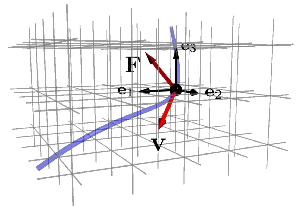
\includegraphics[hiresbb]{./figuras/espacio_base_R3+0_0.pdf}\hss}%
\includemedia[noplaybutton,3Dlights=Headlamp,3Dmenu,3Dtoolbar=false,label=espacio_base_R3,3Daac=33.884454869,3Dc2w=0.894427191 -0.447213595 0 -0.059467182 -0.118934365 0.991119706 -0.443242207 -0.886484414 -0.132972662 69.393365367 153.427432605 16.445624788,3Droo=168.720852518,3Dpsob=H,3Dbg=1 1 1,add3Djscript=asylabels.js]{\phantom{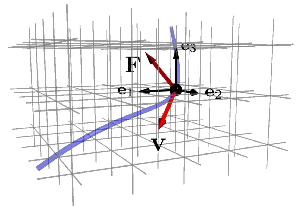
\includegraphics[hiresbb]{./figuras/espacio_base_R3+0_0.pdf}}}{./figuras/espacio_base_R3+0.prc}}%

    \caption{Partícula en \(\mathbb{R}^3\) que sigue una trayectoria (azul) con velocidad \(\mathbf{v}\) y está sometida a la fuerza \(\mathbf{F}\). Sobre la partícula se dibujan los vectores de la base \(\{\mathbf{e}_i\}_{i=1}^3\).}
    \label{fig.1-espacio_base_R3}
\end{figure}

La \cref{fig.1-espacio_base_R3} ilustra la situación estándar de la mecánica newtoniana. Una partícula vive en \(\mathbb{R}^3\), representado mediante las líneas coordenadas en gris, definidas por \(x^i=\text{constante}\). La partícula se mueve con velocidad \(\mathbf{v}\) y está sujeta a la acción de la fuerza \(\mathbf{F}\), ambas indicadas con flechas rojas que nacen de la propia partícula. Además, sobre la posición de la partícula hay una base de tres vectores \(\mathbf{e}_i\), con \(i=1, 2, 3\). Gracias a la base que hemos escogido, podemos expresar las magnitudes vectoriales como
\begin{equation}
    \label{eq.1-sumatorio}
    \mathbf{F} = \sum_{i=1}^3 F^i \mathbf{e}_i \text{  y  } \mathbf{a} = \sum_{i=1}^3 a^i \mathbf{e}_i.
\end{equation}

Aprovechamos este primer ejemplo sencillo para introducir la notación de Einstein.\rnote{Notación de suma de Einstein}{Una expresión con un subíndice y superíndice con el mismo nombre representa la suma sobre dicho índice. Se dice que el índice está contraído.} Es una de esas cosas que al principio le hacen a uno fruncir el ceño, pero que, con el tiempo, se hace querer. Consiste en que, cuando tengamos expresiones con sumatorios como en la \cref{eq.1-sumatorio}, omitiremos el símbolo de sumatorio:
\begin{equation}
    \label{eq.1-einstein}
    \mathbf{F} = F^i \mathbf{e}_i \text{  y  } \mathbf{a} = a^i \mathbf{e}_i.
\end{equation}
A estas alturas puede parecer una frivolidad, pero resulta tan conveniente y cómoda en física que vale la pena ir acostumbrándose a la notación de Einstein. Lo iremos viendo a medida que avanzamos. En cualquier caso, la \cref{eq.1-newton} se traduce en la siguiente relación entre las componentes de los vectores:
\begin{equation}
    F^i = m a^i,
\end{equation}
que dice lo mismo que la \cref{eq.1-newton}, pero escrito de una manera más común en geometría diferencial.\footnote{Por lo menos en la notación de los físicos.}

Antes de proseguir, debemos señalar algo en las expresiones anteriores: la posición de los índices no es tan arbitraria como parece.\rnote{Covariante vs. contravariante}{Nomenclatura habitual en física para referirse al modo de transformación de determinados objetos bajo cambios de base o coordenadas.} De hecho, no es nada arbitraria. Las componentes se han denotado con superíndices (contravariantes), mientras que los vectores de la base llevan subíndices (covariantes). Aún es pronto para apreciar los motivos, pero tiene que ver con cómo se transforman estos objetos cuando se hace un cambio de base. De momento basta quedarse con que la notación de índices no es baladí; está cargada de significado.

Para ``resolver la física'', debemos relacionar las componentes \(F^i\) y \(a^i\) con las coordenadas del punto en el que se encuentra la partícula en un instante dado. Como hemos dicho, nuestra partícula vive en el espacio \(\mathbb{R}^3\), así que tenemos tres coordenadas cartesianas que dependen del tiempo de forma desconocida, \(x^i(t)\). La aceleración es \(a^i = \ddot{x}^i\), mientras que la fuerza depende del sistema concreto que se considere; en general, \(F^i(x^1, x^2, x^3)=F^i(x^j)\). Todo ello nos lleva a un sistema de ecuaciones diferenciales ordinarias (EDOs), cuyas soluciones son las propias coordenadas de la partícula a lo largo de su trayectoria, \(x^i(t)\). A esto se reduce esencialmente toda la física newtoniana, donde las expresiones de \(F^i(x^j)\), junto con las condiciones iniciales, determinan los procesos físicos que sufre la partícula. Asimismo, la generalización a un sistema de partículas es conceptualmente trivial.

\begin{observation}{El vector posición no existe}
    \label{obs.1-no_vector_posicion}
    El título de esta primera observación puede resultar impactante. Sin embargo, lo cierto es que hemos descrito la mecánica newtoniana sin hablar en ningún momento del vector posición, ubicuo en textos introductorios y no tan introductorios de física. En su lugar, hemos relacionado la posición con coordenadas, etiquetas numéricas que identifican puntos dentro del espacio base, reservando el término ``vector'' para cantidades como la velocidad o la fuerza. 
    
    Entonces, ¿por qué hablamos de vector posición normalmente? Resulta que el espacio \(\mathbb{R}^3\), escenario habitual de los problemas de física, tiene la peculiaridad de que sí se puede entender como un espacio vectorial, si se quiere. Basta con definir una suma y un producto por escalares que cumplan las propiedades del álgebra lineal. En este caso sí podemos hablar del vector posición, cuyas componentes son las coordenadas que podemos sumar y restar. ¿Qué pasa en otros espacios?
    
    Imaginemos que nuestra partícula vive en la superficie de una esfera, denotada por \(S^2\). Con esto queremos decir que la partícula no puede salir de la superficie, ya sea porque la forzamos por medios físicos en nuestro universo o porque la partícula existe en un universo imaginario que tiene la forma de \(S^2\). ¿Qué sentido tiene entonces sumar o restar puntos en una esfera? ¿Qué significa tomar un punto de la esfera y multiplicarlo por un escalar?
    
    \begin{figbox}{Partícula en \(S^2\) que sigue una trayectoria (azul) con velocidad \(\mathbf{v}\) y sometida a una fuerza \(\mathbf{F}\). Sobre la partícula se dibujan los dos vectores de la base del espacio tangente \(\{\mathbf{e}_i\}_{i=1}^2\), y una región cuadrada del plano tangente al espacio base. Las líneas grises representan las curvas coordenadas asociadas a los ángulos polar \(x^1 = \theta\) y azimutal \(x^2 = \phi\).
    \label[figure]{fig.1-espacio_base_S2}}
        \setlength{\unitlength}{1pt}%
\makeatletter%
\let\ASYencoding\f@encoding%
\let\ASYfamily\f@family%
\let\ASYseries\f@series%
\let\ASYshape\f@shape%
\makeatother%
\leavevmode\vbox to 141.519400pt{}%
\kern 148.545630pt%
\special{pdf:0.000000 g}%
\special{pdf:0.000000 G}%
\fontsize{12.000000}{14.400000}\selectfont%
\usefont{\ASYencoding}{\ASYfamily}{\ASYseries}{\ASYshape}%
\ASYalign(-74.272815,70.759700)(-0.500000,-0.500000){\hbox to 0pt{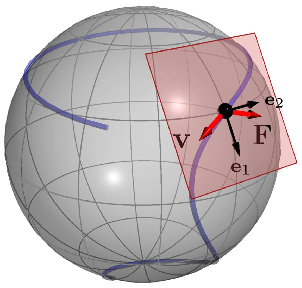
\includegraphics[hiresbb]{./figuras/espacio_base_S2+0_0.pdf}\hss}%
\includemedia[noplaybutton,3Dlights=Headlamp,3Dmenu,3Dtoolbar=false,label=espacio_base_S2,3Daac=22.14342744,3Dc2w=0.389418342 -0.921060994 0 -0.342073466 -0.144626342 0.928476691 -0.855183664 -0.361565854 -0.371390676 303.911139592 132.656914717 132.675377691,3Droo=355.334135857,3Dpsob=H,3Dbg=1 1 1,add3Djscript=asylabels.js]{\phantom{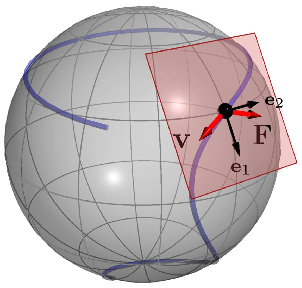
\includegraphics[hiresbb]{./figuras/espacio_base_S2+0_0.pdf}}}{./figuras/espacio_base_S2+0.prc}}%

    \end{figbox}

    Tristemente, al espacio \(S^2\) no se lo puede dotar de estructura de espacio vectorial.\footnote{Esto no es realmente cierto. Hay maneras de dotar a \(S^2\) de estructura vectorial usando herramientas de topología y teoría de conjuntos. Sin embargo, para establecer dicha estructura vectorial, lo único que importa es la cardinalidad (la cantidad de elementos) de \(S^2\); no guarda relación con ninguna propiedad geométrica de la esfera. Se puede encontrar más información buscando el argumento de ``intercalado de dígitos'', \textit{digit interleaving} en inglés, de Cantor.} En espacios así, debemos resignarnos a no hablar del vector posición, sino de coordenadas. A estas alturas puede parecer una distinción superflua, pero lo cierto es que apunta al corazón del análisis tensorial estudiado en geometría diferencial: muchos objetos tienen índices, pero no todos se comportan del mismo modo.
\end{observation}

% \newpage
\begin{observation}{Los vectores son tangentes al espacio base}
    \label{obs.1-espacio_tangente}
    Aparentemente, la observación anterior supone una dificultad para hablar del vector velocidad. Si el espacio base es \(\mathbb{R}^3\) y la partícula se mueve según la trayectoria dada por \(\mathbf{r}(t)\), entonces escribimos 
    \begin{equation}
        \mathbf{v} = \dot{\mathbf{r}} = \lim_{\Delta t\rightarrow0}\frac{\mathbf{r}(t+\Delta t) - \mathbf{r}(t)}{\Delta t}.
    \end{equation}
    Aquí restamos dos vectores posición para llegar a la velocidad. ¿Cómo podemos, entonces, definir el vector velocidad cuando no hay vector posición? 
    
    La clave del asunto es la siguiente: si el espacio base es suficientemente parecido a \(\mathbb{R}^n\),\rnote{Localmente homeomorfo}{Relación topológica entre dos espacios que convierte regiones de uno en regiones del otro mediante deformaciones suaves. Una variedad es suficientemente parecida a \(\mathbb{R}^n\) si es localmente homeomorfa a \(\mathbb{R}^n\).} entonces podemos asignarle un sistema de coordenadas. No nos preocupamos, de momento, por los detalles de las coordenadas.\footnote{Ser precisos con la ``manera apropiada'' de dar coordenadas involucra conocimientos de topología que en esta sección no pintan nada. Nos basta quedarnos con la idea de que podemos dar coordenadas a espacios que sean suficientemente parecidos a \(\mathbb{R}^n\), y ya aclararemos más adelante qué significa ``suficientemente parecidos''.} Basta con la intuición gráfica que viene de imaginar curvas coordenadas como los meridianos y paralelos en la \cref{fig.1-espacio_base_S2}, extendido a otros espacios. Estas coordenadas, como apuntábamos al inicio de la sección, son números reales que sí pueden restarse y sumarse. Ahora, a partir de trayectorias en el espacio base, vamos a lograr construir una estructura vectorial en cada punto del mismo.

    Consideremos un punto \(P\) en \(S^2\), eligiendo coordenadas \(x^1=\theta\) y \(x^2=\phi\), y tomemos distintas trayectorias que pasen por \(P\), como en la \cref{fig.1-trayectorias_tangente_S2}. Cada trayectoria se puede describir convirtiendo las coordenadas en funciones de un parámetro \(t\), \(x^i(t)\), de modo que las coordenadas de \(P\) sean \(x^i(t_0)\) para cierto \(t_0\). Como funciones de variable real que son, podemos tomar la derivada y definir el objeto \(\mathbf{v}\), cuyas componentes son \(v^i(t_0) := \dot{x}^i(t_0)\) en \(P\).

    \begin{figbox}{
        Espacio \(S^2\) con tres puntos resaltados, \(P\), \(P'\) y \(P''\). En cada punto se dibujan dos trayectorias (azul) con velocidades indicadas por flechas rojas. Visualmente se aprecia que las velocidades pertenecen a los planos tangentes, en rojo transparente, que son espacios vectoriales.
        \label{fig.1-trayectorias_tangente_S2}}
        \setlength{\unitlength}{1pt}%
\makeatletter%
\let\ASYencoding\f@encoding%
\let\ASYfamily\f@family%
\let\ASYseries\f@series%
\let\ASYshape\f@shape%
\makeatother%
\leavevmode\vbox to 141.519400pt{}%
\kern 148.545630pt%
\special{pdf:0.000000 g}%
\special{pdf:0.000000 G}%
\fontsize{12.000000}{14.400000}\selectfont%
\usefont{\ASYencoding}{\ASYfamily}{\ASYseries}{\ASYshape}%
\ASYalign(-74.272815,70.759700)(-0.500000,-0.500000){\hbox to 0pt{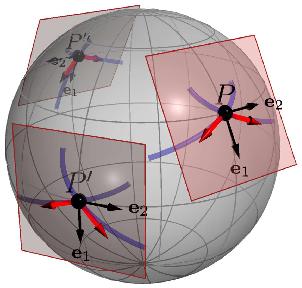
\includegraphics[hiresbb]{./figuras/trayectorias_tangente_S2+0_0.pdf}\hss}%
\includemedia[noplaybutton,3Dlights=Headlamp,3Dmenu,3Dtoolbar=false,label=trayectorias_tangente_S2,3Daac=22.256194492,3Dc2w=0.389418342 -0.921060994 0 -0.342073466 -0.144626342 0.928476691 -0.855183664 -0.361565854 -0.371390676 301.584004652 131.78689251 132.538343984,3Droo=353.492320709,3Dpsob=H,3Dbg=1 1 1,add3Djscript=asylabels.js]{\phantom{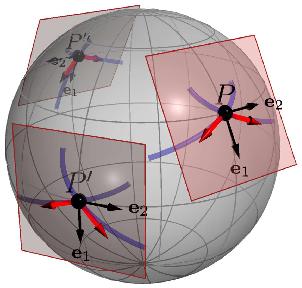
\includegraphics[hiresbb]{./figuras/trayectorias_tangente_S2+0_0.pdf}}}{./figuras/trayectorias_tangente_S2+0.prc}}%

    \end{figbox}

    Demostrar explícitamente que las \(\mathbf{v}\)'s forman un espacio vectorial no es importante en este momento. Sí que hay que quedarse con la intuición visual mostrada en la \cref{fig.1-trayectorias_tangente_S2}, donde las flechas rojas se corresponden con las velocidades de las trayetorias azules. Además, por ser la velocidad tangente a la trayectoria, el conjunto de las \(\mathbf{v}\)s formará un espacio tangente a \(S^2\) en \(P\).
    Claramente, las \(\mathbf{v}\)'s tienen las propiedades elementales de los vectores dentro del espacio tangente: módulo, dirección y sentido. 
    
    Parece, pues, razonable usar estos objetos para construir un espacio vectorial asociado al punto \(P\). Es más, el punto \(P\) no tiene nada de especial; hay muchos otros en \(S^2\) con el mismo derecho a que les presten atención. Repitiendo el análisis para cada punto de \(S^2\), llegaríamos a\rnote{Fibrado tangente}{La unión de todos los espacios tangentes se denota como fibrado tangente, y es un primer ejemplo de la familia de objetos conocidos como fibrados, \textit{bundle} en inglés.} una familia de espacios tangentes independientes. En la \cref{fig.1-trayectorias_tangente_S2} se muestran tres, pero realmente hay infinitos de ellos.
    
    Las dos observaciones anteriores nos han llevado a un momento idóneo para hacer otro comentario que puede resultar chocante. Si queremos restar dos vectores que pertenecen al mismo espacio vectorial no hay duda; los restamos y punto. En cambio, si los vectores pertenecen a espacios tangentes distintos, como en la \cref{fig.1-trayectorias_tangente_S2} ya no está tan claro. Desde luego, no podemos restarlos al tuntún. Al fin y al cabo, pertenecen a espacios vectoriales distintos. ¿Cómo podemos, pues, comparar velocidades en puntos distintos del espacio base? ¿O comparar vectores, en general? Hasta donde hemos visto, son churras y merinas. Entre otras cosas, en este curso vamos a aprender a dar sentido a la comparación de vectores que viven en espacios tangentes distintos.\rnote{Conexión afín}{Objeto eminentemente geométrico que relaciona consistentemente espacios tangentes entre puntos distintos. Es fundamental en geometría diferencial.}
    
    He aquí otro efecto pernicioso de trabajar en \(\mathbb{R}^3\), igual que con el asunto del vector posición. Hasta ahora hemos restado vectores que actúan en puntos distintos sin miramientos. Lo podemos hacer en \(\mathbb{R}^3\) porque existe una identificación canónica de traslación entre los espacios tangentes. En otros espacios base, sin embargo, debemos profundizar un poco más. Una explicación detallada sería prematura, pero así hay algo más que esperar con ilusión.
    
\end{observation}

\subsection{Transformación de coordenadas y cambio de base}
\label{subsec.1transformaciones}

Ha quedado establecido que existe una diferencia entre coordenadas y vectores. Además, el espacio tangente donde viven los vectores es formalmente independiente del espacio base donde viven las posiciones. Se deduce que, en general, la base escogida en el espacio tangente y las coordenadas que cubren el espacio base no tienen por qué estar relacionadas. Aun así, es muy común y conveniente escoger una base adecuada a las coordenadas. Ya hemos visto ejemplos en \(\mathbb{R}^3\) de distintos sistemas de coordenadas (cartesianas, esféricas y cilíndricas) y sus bases asociadas.

Una pregunta natural para lectores atentos es la siguiente: ¿cómo cambian los vectores de la base si cambio de coordenadas? ¿Hay alguna expresión compacta? ¿Y las coordenadas de un vector arbitrario? Preguntas fascinantes, qué duda cabe. Aquí vamos a poner un tráiler mostrando varios ejemplos típicos, y no tan típicos. Siguiendo la tónica de esta introducción, no vamos a demostrar aún por qué las cosas son como son. Esta sección solo busca ser suficientemente convincente.

\begin{example}{Coordenadas rectilíneas en \(\mathbb{R}^2\)}
    \label{ex.1-plano_coordenadas_rect}
    En este primer ejemplo tomamos dos sistemas de coordenadas, \(x^i\) y \(x^{i'}\), ilustradas por las líneas grises y rojo claro de la \cref{fig.1-plano_coordenadas_rect}. Las primeras son las coordenadas cartesianas de toda la vida, mientras que las segundas son el resultado de estirar y rotar las cartesianas. Son menos bonitas, claro, pero igualmente válidas para especificar puntos en el plano.
    \begin{align}
        \label{eq.1-transformacion_coordenadas_ejemplo1}
        \left\{\begin{aligned}
            x^1 &= x \\
            x^2 &= y
        \end{aligned} \right. \quad \text{y} \quad
        \left\{\begin{aligned}
            x^{1'} &= \frac{1}{3}x + \frac{2}{3}y \\
            x^{2'} &= -\frac{2}{3}x + \frac{2}{3}y
        \end{aligned} \right. \implies 
        \left\{
        \begin{aligned}
            x^{1'} &= \frac{1}{3}x^1 + \frac{2}{3}x^2 \\
            x^{2'} &= -\frac{2}{3}x^1 + \frac{2}{3}x^2
        \end{aligned}\right..
    \end{align}
    Hemos quitado ya la muleta de \(x\) e \(y\) para quedarnos solo con la notación general de la transformación de coordenadas.\marginexercise[-2cm]{Todo aquel que lea estas notas debería dedicar unos minutos a intentar obtener esta ley de transformación a partir de la \cref{fig.1-plano_coordenadas_rect}.}

    \begin{figbox}{Líneas coordenadas de \(x^i\) (cartesianas, en gris) y \(x^{i'}\) (menos bonitas, rojo claro), definidas por \(x^{i}=0,\pm1, \pm2, \pm3\) y \(x^{i'}=0,\pm1, \pm2, \pm3\), respectivamente. Con línea más gruesa y color más intenso, se representan los vectores de las bases asociadas a las coordenadas: \(\mathfrak{B} = \{\mathbf{e}_i\}_{i=1}^2\) y \(\mathfrak{B}' = \{\mathbf{e}_{i'}\}_{i=1}^2\).
    \label{fig.1-plano_coordenadas_rect}}
    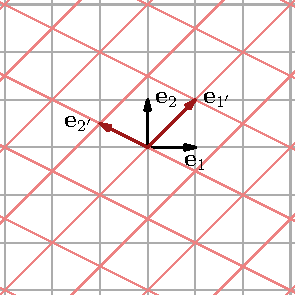
\includegraphics{figuras/plano_coordenadas_rect.pdf}
    \end{figbox}

    Dadas estas coordenadas \(x^i\) y \(x^{i'}\), definimos sendas bases de vectores del espacio tangente,\footnote{Sí, como estamos en \(\mathbb{R}^2\), el espacio tangente es, en cierto sentido, indistinguible del propio espacio base. Aun así, son conceptualmente distintos.} \(\mathfrak{B} = \{\mathbf{e}_i\}_{i=1}^2\) y \(\mathfrak{B}' = \{\mathbf{e}_{i'}\}_{i=1}^2\), representadas en \cref{fig.1-trayectorias_tangente_S2}, Para pasar de una base a la otra, aplicamos una ``matriz de cambio de base'', \(\mathbf{T}\). Ante las matrices de cambio de base del álgebra elemental hay una duda recurrente para quienes tienen mala memoria. ¿Dónde va \(\mathbf{T}\) y dónde \(\mathbf{T}^{-1}\)? ¿Está formada \(\mathbf{T}\) por las componentes de los vectores \(\mathbf{e}_{i'}\) en la base \(\mathfrak{B}\) o al revés? Aquellos que se ven atormentados por este tipo de preguntas respirarán aliviados cuando terminemos el ejemplo. Nunca más van a tener que recordar esos detalles, siempre y cuando conozcan la regla que vamos a dar a continuación.

    En primer lugar,\marginexercise{Es más fácil de ver, pero también es recomendable darle una vuelta a la \cref{eq.1-transformacion_vectores_ejemplo1}.} como los números se han escogido para que sea sencillo, a partir de la \cref{fig.1-plano_coordenadas_rect} se deduce que
    \begin{equation}
        \label{eq.1-transformacion_vectores_ejemplo1}
        \mathbf{e}_{1'} = 1 \mathbf{e}_{1} + 1 \mathbf{e}_{2}\quad \text{y} \quad\mathbf{e}_{2'} = -1 \mathbf{e}_{1} + \frac12 \mathbf{e}_{2}.
    \end{equation}
    ¿Qué relación guarda la \cref{eq.1-transformacion_vectores_ejemplo1} con la \cref{eq.1-transformacion_coordenadas_ejemplo1}? Es evidente que si cambio las líneas de coordenadas, también cambian los vectores asociados; tiene que haber alguna relación entre las \cref{eq.1-transformacion_vectores_ejemplo1,eq.1-transformacion_coordenadas_ejemplo1}. Pues bien, la relación es
    \begin{bequation}
        \label{eq.1-transformacion_vectores}
        \mathbf{e}_{i'} = \jcbn{x}{i}{x}{i'}\mathbf{e}_i,
    \end{bequation}
    ni más ni menos.\footnote{Puede parecer que nos la hemos sacado de la manga, y es que así ha sido, efectivamente. En las \cref{sec.2tensores,sec.3variedades} explicaremos de dónde viene.} Ojo, en el lado derecho, estamos sumando el índice \(i\), de acuerdo con la notación de Einstein. Como está sumado, se dice que el índice \(i\) es ``mudo'', y el único que queda ``libre'' es el \(i'\), que aparece en ambos lados como subíndice. 
    
    Vamos a desarrollar las derivadas parciales, a ver si, en efecto, recuperamos \cref{eq.1-transformacion_vectores_ejemplo1}. El problema que encontramos es que tenemos \(x^{i'}(x^i)\), pero lo que necesitamos es \(x^i(x^{i'})\). Hay que invertir la \cref{eq.1-transformacion_coordenadas_ejemplo1}. Por un lado, restando \(x^{1'}\) y \(x^{2'}\) llegamos a \(x^1 = x^{1'}-x^{2'}\). Por otro, multiplicando \(x^{2'}\) por \(1/2\) y sumando \(x^{1'}\) obtenemos \(x^2 = x^{1'}+\frac12x^{2'}\). Así, las \rnote{Matriz jacobiana}{De los cursos iniciales de cálculo, la matriz jacobiana de una transformación de coordenadas nos permite estudiar su aspecto lineal local. Realmente aquí usamos los elementos de la matriz jacobiana inversa.} derivadas parciales quedan
    \begin{equation*}
         \jcbn{x}{1}{x}{1'} = 1, 
        \quad  \jcbn{x}{1}{x}{1'} = 1,
        \quad  \jcbn{x}{1}{x}{1'} = -1\quad \text{y}
        \quad  \jcbn{x}{1}{x}{1'} = \frac12.
    \end{equation*}
    Con estas, desempaquetamos la suma implícita de la \cref{eq.1-transformacion_vectores} y llegamos justo a la \cref{eq.1-transformacion_vectores_ejemplo1}. Parece que funciona. Con un poquito de esfuerzo, seguro que podríamos llegar de la \cref{eq.1-transformacion_coordenadas_ejemplo1} a la \cref{eq.1-transformacion_vectores_ejemplo1} sin pasar por la \cref{eq.1-transformacion_vectores}, ciertamente. De todos modos, este es el ejemplo más simple de todos; en los siguientes no está tan claro.
\end{example}

\begin{observation}
    {Vectores con componentes en \(\mathbb{R}^2\)}
    \label{obs.1-vectores_componentes}
    El ejemplo anterior da pie a discutir brevemente la otra cara de la moneda en lo que respecta a transformaciones de coordenadas y cambios de base. Hemos comprobado que la \cref{eq.1-transformacion_vectores} nos da la relación de los vectores de una base a la otra, por lo menos en ese caso sencillo. Vamos a creérnosla, de momento. 

    Ahora bien, damos la lata con los vectores de la base porque son muy útiles; nos permiten construir cualquier otro mediante combinaciones lineales. Supongamos que tenemos un vector \(\mathbf{w}\) que se expresa como \(\mathbf{w} = w^i \mathbf{e}_i\),\footnote{¡Notación de Einstein! Llegará un momento donde ya no lo advertiremos... Más vale ir acostumbrándose.} donde \(w^i\) son las componentes de \(\mathbf{w}\) en la base \(\mathfrak{B}\). La pregunta que debemos plantearnos es la siguiente. Si sabemos cómo cambian los vectores de la base, ¿cómo cambian las componentes de un vector cualquiera? Es decir, si usamos la base \(\mathfrak{B}'\) y escribimos \(\mathbf{w} = w^{i'}\mathbf{e}_{i'}\), ¿cuál es la relación entre \(w^{i'}\) y \(w^i\)?

    Resulta que hay una versión de la \cref{eq.1-transformacion_vectores} para componentes:
    \begin{bequation}
        \label{eq.1-transformacion_componentes}
        w^{i'} = \jcbn{x}{i'}{x}{i} w^{i}.
    \end{bequation}
    La diferencia respecto a la \cref{eq.1-transformacion_vectores} es que aquí la coordenada \(x^{i'}\) se deriva respecto a la coordenada \(x^{i}\). Por tanto, aparecen los elementos de la matriz Jacobiana, en lugar de la inversa como aparecen en la transformación de los vectores. 
    
    Fijémonos en un detalle. Tanto en la \cref{eq.1-transformacion_vectores} como en la \cref{eq.1-transformacion_componentes}, la propia estructura de índices nos dice dónde va qué matriz de transformación; no hace falta aprendérselo de memoria. Si a la izquierda el índice \(i'\) va abajo, como la \cref{eq.1-transformacion_vectores}, a la derecha también abajo, con lo que la posición de \(i\) queda fija automáticamente. Lo contrario si a la izquierda el índice \(i'\) va arriba. Y la posición de los índices la determina el tipo de objeto estemos transformando. ¡Todo cuadra!

    Hay una forma interesante de entender la \cref{eq.1-transformacion_componentes} a partir de la \cref{eq.1-transformacion_vectores}, o viceversa. La cuestión es que, sea cual sea la base que usemos, el objeto \(\mathbf{w}\) no cambia. Lo que cambian son sus componentes, pero \(\mathbf{w}\) siempre apunta en la misma dirección y tiene el mismo módulo. Es como decir ``Hola, ¿quién eres?'' o ``Hallo, wer bist du?''; mismo mensaje, distinta lengua. Entonces, 
    \begin{align}
        \nonumber
        \mathbf{w} &= w^{i'}\mathbf{e}_{i'} = 
        \jcbn{x}{i'}{x}{j} w^j 
        \jcbn{x}{k}{x}{i'} \mathbf{e}_k 
        = \jcbn{x}{k}{x}{i'} \jcbn{x}{i'}{x}{j} w^j \\
        \label{eq.1-vectores_invariantes}
        &= \jcbn{x}{k}{x}{j} w^j \mathbf{e}_k 
        = {\tensor{\delta}{^k_j}} w^j \mathbf{e}_k = w^k \mathbf{e}_k.
    \end{align}
    Aquí hay bastante que desempaquetar;\rnote[-0.8cm]{Delta de Kronecker}{\(\tensor{\delta}{^i_j}\) son las componentes de un tensor de rango \((1, 1)\). Vale 1 cuando \(i=j\), y 0 cuando \(i\neq j\) y representa la matriz identidad. Aquí aparece porque estamos haciendo la multiplicación de la matriz jacobiana y su inversa (equivalentemente, por la regla de la cadena).} vayamos paso a paso. 
    
    En primer lugar, hemos usado las \cref{eq.1-transformacion_vectores,eq.1-transformacion_componentes}. Atención con los nuevos índices \(j\) y \(k\). Se refieren a sumas distintas, así que deben llevar nombres diferentes. Luego, hemos reordenado los términos. Podemos hacerlo porque, con los sumatorios implícitos, realmente solo escribimos un sumando arbitrario de todos los que realmente hay. Dicho sumando está compuesto por dos derivadas parciales, una componente y un vector, es decir, números y un vector multiplicados. El siguiente paso es más interesante: la regla de la cadena del cálculo multivariable,\marginexercise[-2cm]{Será muy importante para nosotros, así que quien no tenga clara la regla de la cadena multivariable debería entender esto como un aviso para revisarla.} que nos permite eliminar el índice mudo \(i'\). A continuación, las coordenadas son funciones independientes; si me muevo en una dirección, no avanzo nada en otra. Por tanto \(\jcbn{x}{k}{x}{j}\) es 1 cuando \(j=k\), y 0 cuando \(j\neq k\). Habitualmente denotamos esa situación por \(\tensor{\delta}{^k_j}\), la \(\delta\) de Kronecker. Por último, la suma implícita sobre \(j\)\marginexercise{La primera vez puede no estar claro, pero es muy importante convencerse de que \(\tensor{\delta}{^k_j}w^j = w^k\).} con la \(\delta\) de Kronecker elimina todos los sumandos en \(j\) que no sean justo aquellos en los que \(j=k\).
\end{observation}

\begin{example}{Coordenadas cartesianas y polares en \(\mathbb{R}^2\)}
    \label{ex.1-plano_coordenadas_polar}
    Nos mantenemos en el espacio base de \(\mathbb{R}^2\), tan sencillo como en el primer ejemplo, pero ahora damos coordenadas cartesianas y polares:
    \begin{align}
        \label{eq.1-transformacion_coordenadas_ejemplo2}
        \left\{\begin{aligned}
            x^{1'} &= \sqrt{(x^1)^2 + (x^2)^2} \\
            x^{2'} &= \arctan\left(\frac{x^2}{x^1}\right)
        \end{aligned}\right. \iff
        \left\{\begin{aligned}
            x^{1} &= x^{1'}\cos\left(x^{2'}\right) \\
            x^{2} &= x^{1'}\sin\left(x^{2'}\right) 
        \end{aligned}\right..
    \end{align}
    Por supuesto, \(x^{1'}\) es la variable radial \(r\) y \(x^{2'}\) la angular \(\theta\). La \cref{fig.1-plano_coordenadas_polar} presenta las líneas coordenadas respectivas. Comparando con la \cref{fig.1-plano_coordenadas_rect}, nada cambia respecto a las grises, pero las rojas ahora tienen más miga. Hay líneas circulares (\(x^{1'} = r = \text{const.}\)) y radiales (\(x^{2'} = \theta = \text{const.}\)).
    
    Asociadas a cada sistema de coordenadas, de nuevo dibujamos una base de vectores. Dada la forma curvilínea de las coordenadas polares, cada punto tendrá sus propia base de vectores asociados. Para ilustrarlo, la \cref{fig.1-plano_coordenadas_polar} destaca dos puntos de \(\mathbb{R}^2\). Como es de esperar, los vectores cartesianos \(\mathbf{e}_i\), en negro, son iguales en ambos puntos. En cambio, los vectores polares \(\mathbf{e}_{i'}\) cambian de un punto a otro. En primer lugar, los vectores polares rotan de manera que \(\mathbf{e}_{1'}|_P\)\footnote{La notación \(f|_x\) denota la función \(f\) evaluada en \(x\). En este caso, la función que evaluamos es el propio vector de la base polar en el punto \(P\).} siempre es radial en cada punto \(P\), y \(\mathbf{e}_{2'}|_P\) siempre apunta en la dirección angular.

    \begin{figbox}
        {Líneas coordenadas de \(x^i\) (cartesianas, en gris) y de \(x^{i'}\) (polares, rojo claro). En dos puntos, se representan los vectores de las bases coordenadas (negro: vectores cartesianos, rojo: vectores polares). Los vectores polares cambian su orientación y su módulo en función del punto que se considere.
        \label{fig.1-plano_coordenadas_polar}}
        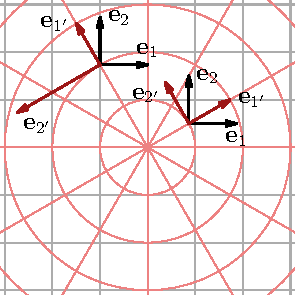
\includegraphics{figuras/plano_coordenadas_polar.pdf}
    \end{figbox}
    
    Con un poco de trigonometría y voluntad, podríamos obtener la expresión de los vectores polares en términos de los vectores cartesianos. Otra opción, más alineada con este curso, es volver a usar la \cref{eq.1-transformacion_vectores}. Las derivadas importantes ahora son\marginexercise{Es instructivo hacer también la transformación en sentido contrario, es decir, expresar los vectores cartesianos en términos de los vectores polares utilizando, de nuevo, la \cref{eq.1-transformacion_vectores}.}
    \begin{align*}
        \jcbn{x}{1}{x}{1'} &= \cos\left(x^{2'}\right), & &&  \jcbn{x}{2}{x}{1'} &= \sin\left(x^{2'}\right),\\
        \jcbn{x}{1}{x}{2'} &= -x^{1'}\sin\left(x^{2'}\right) & \text{y} &&
        \jcbn{x}{1}{x}{1'} &= x^{2'}\cos\left(x^{2'}\right),
    \end{align*}
    Con ellas, llegamos a 
    \begin{align}
        \left\{\begin{aligned}
            \mathbf{e}_{1'} &= \cos\left(x^{2'}\right) \mathbf{e}_{1} + \sin\left(x^{2'}\right) \mathbf{e}_{2}
            \ \text{y}\\
            \mathbf{e}_{2'} &= -x^{1'}\sin\left(x^{2'}\right) \mathbf{e}_{1} + x^{1'}\cos\left(x^{2'}\right) \mathbf{e}_{2}.
        \end{aligned}\right.
    \end{align}
    A diferencia del primer ejemplo, ahora los coeficientes de la transformación dependen de la posición. Hemos expresado esta dependencia con las coordenadas polares \(x^{i'}\), pero podríamos sin ningún problema tomar la \cref{eq.1-transformacion_coordenadas_ejemplo2} para convertir los coeficientes en términos de las coordenadas cartesianas.\marginexercise{Para ir calentando la muñeca, un ejercicio sencillo es expresar los coeficientes como funciones de las coordenadas cartesianas.}
\end{example}

\begin{observation}
    {Las bases coordenadas no son ortonormales}
    \label{obs.1-bases_no_ortonormales}
    Un aspecto interesante que se desprende de los dos ejemplos anteriores es que las bases de vectores dados por las coordenadas no son necesariamente ortonormales. En el primer ejemplo (\cref{fig.1-plano_coordenadas_rect}), los vectores \(\mathbf{e}_{1'}\) y \(\mathbf{e}_{2'}\) son claramente no ortogonales.\marginexercise{Otro buen ejercicio de calentamiento es obtener el producto escalar de \(\mathbf{e}_{1'}\) y \(\mathbf{e}_{2'}\) en el \cref{ex.1-plano_coordenadas_rect}, así como sus módulos.} Esto es consecuencia de que las líneas coordenadas no forman ángulos de 90 grados, y de que para llegar de una línea a la siguiente necesito avanzar más de 1 unidad.

    Por otro lado, en el segundo ejemplo los vectores polares sí son ortogonales, pero el módulo de vector angular \(\mathbf{e}_{2'}\) es igual a la coordenada radial \(x^{1'}\). Puede parecer un poco raro, pero cobra bastante sentido si recordamos que los vectores los definimos a partir de velocidades de trayectorias. Imagina la trayectoria circular dada por \(x^{1'}(t)=r_0\) y \(x^{2'}(t)=t\). A medida que avanza \(t\), la trayectoria recorre una circunferencia de radio \(r_0\). Cuando \(t\) barre el intervalo \([0, 2\pi]\), la trayectoria completa una vuelta entera. ¿Qué distancia total se ha recorrido? \(2\pi r_0\). ¿En cuánto \(t\)? \(2\pi\). El vector velocidad asociado debe, entonces, tener módulo \(r_0\). De alguna manera tiene que compensar el hecho de que \(x^{2'}\) (\(\theta\)) ``no sabe nada sobre \(x^{1'}\) (\(r\))'', pero no es lo mismo dar vueltas my cerca del origen que darlas muy lejos.
\end{observation}

Con estos dos ejemplos y observaciones ya hemos visto todo lo importante de esta sección. Aun así, vamos a añadir un ejemplo más con la excusa de salirnos del plano, que es nuestro objetivo al fin y al cabo.

\begin{example}
    {Coordenadas de proyección y esféricas en \(S^2\)}
    \label{ex.1-hemisferio_norte_S2}
    Vamos a volver a considerar \(S^2\), restringido esta vez al hemisferio norte, con dos sistemas de coordenadas distintos. El primer sistema (\(x^i,\ i=1, 2\)) lo podemos imaginar como el resultado de cortar rebanadas verticales, a lo largo y a lo ancho, con un cuchillo. Los cortes en la superficie de la semiesfera se corresponden con las líneas coordenadas. En una jerga más técnica, este primer sistema de coordenadas viene de considerar \(S^2\) como un espacio bidimensional embebido en \(\mathbb{R}^3\), como la solemos visualizar. Si a \(\mathbb{R}^3\) lo describimos con coordenadas cartesianas \(\left(x^1, x^2, x^3\right)\), lo que estamos haciendo es proyectar sobre el plano \(x^3=0\) para quedarnos con \(x^i,\ i=1, 2\). En la \cref{fig.1-hemisferio_norte_S2}, las curvas coordenadas asociadas a este sistema son las líneas grises. No debería sorprender a nadie que, asociada a \(x^i\), existe una base de vectores tangentes a \(S^2\) representados con flechas negras en la figura. El segundo sistema, representado en rojo, consiste en los ángulos azimutal y polar: \(x^{1'}=\theta\) y \(x^{2'}=\phi\), respectivamente. 

    La transformación de coordenadas es, en ambos sentidos,
    \begin{align}
        \nonumber
        \text{(proyección)}&\left\{\begin{aligned}
            x^1 &= \sin\left(x^{1'}\right)\cos\left(x^{2'}\right)\\
            x^2 &= \sin\left(x^{1'}\right)\sin\left(x^{2'}\right)
        \end{aligned}\right., \\
        \label{eq.1-transformacion_coordenadas_ejemplo3}
        \text{(esféricas)}&\left\{\begin{aligned}
            x^{1'} &= \arccos\left(\sqrt{1-\left(x^1\right)^2-\left(x^2\right)^2}\right)\\
            x^{2'} &= \arctan\left(\frac{x^{2}}{x^{1}}\right)
        \end{aligned}\right. .
    \end{align}
    Es relativamente sencillo visualizar las líneas coordenadas, especialmente con la \cref{eq.1-transformacion_coordenadas_ejemplo3} a nuestra disposición. En cambio, las expresiones concretas de los vectores se hacen un poco más de rogar.
    
    \begin{figbox}
        {Líneas coordenadas y bases asociadas en el hemisferio norte de \(S^2\). Las líneas grises se corresponden con las coordenadas que resultan de proyectar la superficie sobre el plano ecuatorial. Las rojas están ligadas a los ángulos azimutal y polar. En dos puntos se representan las bases de vectores tangentes.
        \label{fig.1-hemisferio_norte_S2}}
        \setlength{\unitlength}{1pt}%
\makeatletter%
\let\ASYencoding\f@encoding%
\let\ASYfamily\f@family%
\let\ASYseries\f@series%
\let\ASYshape\f@shape%
\makeatother%
\leavevmode\vbox to 107.391970pt{}%
\kern 148.545630pt%
\special{pdf:0.000000 g}%
\special{pdf:0.000000 G}%
\fontsize{12.000000}{14.400000}\selectfont%
\usefont{\ASYencoding}{\ASYfamily}{\ASYseries}{\ASYshape}%
\ASYalign(-74.272815,53.695985)(-0.500000,-0.500000){\hbox to 0pt{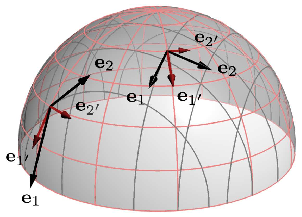
\includegraphics[hiresbb]{./figuras/hemisferio_norte_S2+0_0.pdf}\hss}%
\includemedia[noplaybutton,3Dlights=Headlamp,3Dmenu,3Dtoolbar=false,label=hemisferio_norte_S2,3Daac=16.185188108,3Dc2w=0.389418342 -0.921060994 0 -0.342073466 -0.144626342 0.928476691 -0.855183664 -0.361565854 -0.371390676 316.916786788 130.937408341 155.286569621,3Droo=362.280587463,3Dpsob=H,3Dbg=1 1 1,add3Djscript=asylabels.js]{\phantom{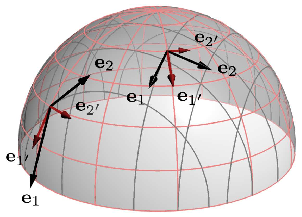
\includegraphics[hiresbb]{./figuras/hemisferio_norte_S2+0_0.pdf}}}{./figuras/hemisferio_norte_S2+0.prc}}%

    \end{figbox}

    Los vectores esféricos \(\mathbf{e}_{i'}\), vistos como elementos de \(\mathbb{R}^3\) se pueden obtener de forma directa en términos de los tres vectores cartesianos de \(\mathbb{R}^3\);\marginexercise{Obtener las componentes de \(\mathbf{e}_{1'}\) y \(\mathbf{e}_{2'}\) (esféricos), en términos de los vectores coordenados cartesianos de \(\mathbb{R}^3\), donde está embebido nuestro espacio base.} solo hay que repetir el análisis del \cref{ex.1-plano_coordenadas_polar}, pero con 3 coordenadas. Lo que queremos hacer, suponiendo que ya tenemos los vectores asociados a las coordenadas esféricas, es obtener los vectores asociados a las coordenadas de proyección. Para ello, volvemos a tomar la \cref{eq.1-transformacion_vectores}, que ya debe ser de nuestras ecuaciones favoritas. Vamos a volver a escribirla, que la letra con sangre entra:
    \begin{equation}
        \mathbf{e}_{i} = \jcbn{x}{i'}{x}{i} \mathbf{e}_{i'}.
    \end{equation}
    Aquí, las derivadas son un poco engorrosas (mira el margen izquierdo).\marginexercise{Calcular estas derivadas parciales es hacer méritos para subir de nivel.} Vamos a poner el resultado:
    \begin{align*}
         \jcbn{x}{1'}{x}{1} &= \frac{x^{1}}{\sqrt{\big((x^1)^2 + (x^2)^2\big)\big(1 - (x^1)^2 - (x^2)^2\big)}}, & &&  \jcbn{x}{2'}{x}{1} &= \frac{x^{1}}{(x^{1})^2 + (x^{2})^2},\\
         \jcbn{x}{1'}{x}{2} &= \frac{x^{2}}{\sqrt{\big((x^1)^2 + (x^2)^2\big)\big(1 - (x^1)^2 - (x^2)^2\big)}}, & \text{y} &&  \jcbn{x}{2'}{x}{2} &= \frac{-x^{2}}{(x^{1})^2 + (x^{2})^2}.
    \end{align*}

    Llegados a este punto, se puede pensar ``y todo esto, ¿para qué?'' No es que hayamos llegado a unas expresiones sencillas al final de todas las cuentas, al fin y al cabo. Hay muchas respuestas posibles para escoger; cada uno puede buscar la suya. Aquí damos la siguiente. Son ejemplos que ilustran bien las ideas y fórmulas generales. Es más, con el \cref{ex.1-hemisferio_norte_S2} se atisba una regla bastante general e incómoda sobre la geometría diferencial ``práctica'': las ideas generales se expresan de forma simple, los casos particulares requieren fórmulas complicadas. Es el precio que hay que pagar por viajar a espacios interesantes. Además, aunque algunas expresiones sean complicadas, también lo es la vida. No va a ser todo planos inclinados y osciladores armónicos; se haría un poco aburrido. 
\end{example}

\begin{observation}
    {No vale con un solo sistema de coordenadas}
    \label{obs.1-atlas}
    El ejemplo anterior es muy completo, porque contiene todo lo que sabemos de geometría diferencial: (i) según el punto en el que se mire, los vectores no son ortogonales ni están normalizados; (ii) el espacio es genuinamente curvo, a diferencia de los ejemplos 1 y 2,\footnote{En el \cref{ex.1-plano_coordenadas_polar} las coordenadas polares son curvilíneas, pero el espacio sigue siendo plano.} y (iii) las expresiones tienen cierta complicación. De todos modos, uno podría preguntarse por qué restringirse al hemisferio norte. Para dar con la respuesta, imaginemos la esfera completa, \(S^2\). Las coordenadas esféricas son casi biyectivas en el sentido de que, a cada par de valores \((\theta, \phi)\) le corresponde un único punto de la esfera, salvo los polos. En efecto, el ángulo polar \(\phi\) no está definido en dichos puntos. Por lo demás, la relación es biunívoca. En cambio, con las coordenadas de la proyección no es así. Solo con el par \((x, y)\) no podemos distinguir entre hemisferios. Tenemos, entonces, dos opciones. La primera es simplemente restringir \(S^2\) a uno de sus hemisferios. La segunda,\rnote{Atlas}{Familia de cartas (sistemas de coordenadas) compatibles que cubren la variedad (espacio base).} más interesante,\marginexercise{Conceptualmente, esbozar distintos atlas posibles para la esfera, el plano o, quien se atreva, algún otro espacio base.} es buscar varios sistemas de coordenadas compatibles que, entre todos, cubran la esfera completa. Los sistemas de coordenadas deben ser compatibles en el sentido de poder cambiar de uno a otro en las regiones de solapamiento. En la \cref{fig.1-atlas_S2} tenemos justo esa situación, con coordenadas rojas y azules que, combinadas, cubren el espacio entero. \marginexercise{Es interesante pensar cómo obtener el cambio de coordenadas en la región de \(S^2\) donde coexisten ambos sistemas de coordenadas.}
    
    \begin{figbox}
        {Ejemplo de atlas para \(S^2\). Las coordenadas rojas son los ángulos esféricos habituales, pero con \(\theta\in[\pi/6, 5\pi/6]\) para evitar el problema en los polos. Otras coordenadas, en azul, cubren los casquetes que faltan. Las coordenadas azules se obtienen rotando \(\pi/2\) alrededor del eje \(Y\) las rojas.
        \label{fig.1-atlas_S2}}
        \setlength{\unitlength}{1pt}%
\makeatletter%
\let\ASYencoding\f@encoding%
\let\ASYfamily\f@family%
\let\ASYseries\f@series%
\let\ASYshape\f@shape%
\makeatother%
\leavevmode\vbox to 148.545630pt{}%
\kern 148.545630pt%
\special{pdf:0.000000 g}%
\special{pdf:0.000000 G}%
\fontsize{12.000000}{14.400000}\selectfont%
\usefont{\ASYencoding}{\ASYfamily}{\ASYseries}{\ASYshape}%
\ASYalign(-74.272815,74.272815)(-0.500000,-0.500000){\hbox to 0pt{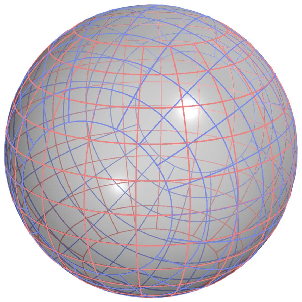
\includegraphics[hiresbb]{./figuras/atlas_S2+0_0.pdf}\hss}%
\includemedia[noplaybutton,3Dlights=Headlamp,3Dmenu,3Dtoolbar=false,label=atlas_S2,3Daac=22.054366812,3Dc2w=0.389418342 -0.921060994 0 -0.342073466 -0.144626342 0.928476691 -0.855183664 -0.361565854 -0.371390676 318.890321844 134.857358722 138.498559132,3Droo=372.906683393,3Dpsob=H,3Dbg=1 1 1,add3Djscript=asylabels.js]{\phantom{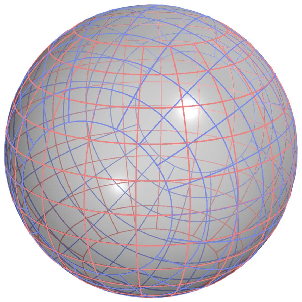
\includegraphics[hiresbb]{./figuras/atlas_S2+0_0.pdf}}}{./figuras/atlas_S2+0.prc}}%

    \end{figbox}
    
\end{observation}

\subsection{Escalares: mecánica lagrangiana}
\label{subsec.1escalares}

Hemos hablado de coordenadas y vectores. Otro tipo de objeto importante, y más sencillo, son los escalares. Un escalar es una función que asigna un valor real a los punto del espacio. Para que nos entendamos, la temperatura en la superficie de la Tierra o la densidad de un medio inhomogéneo. Lo interesante de un escalar es que no tiene componentes, no es más que un número en cada punto. Son tan sencillos que su ley de transformación análoga a las \cref{eq.1-transformacion_vectores,eq.1-transformacion_componentes} es que simplemente no se transforman.\footnote{Si tenemos un escalar \(e\) en el punto \(P\), lo expresamos como función de las coordenadas \(x^i|_P\), \(e(x^i|_P)\). Bajo cambios de coordenadas el punto \(P\) no cambia, pero sus componentes sí. El escalar, en las nuevas coordenadas, se expresa como \(e(x^i(x^{j'}|_P))=:e'(x^{j'})\). En términos prácticos, la función \(e\) cambia por la función \(e'\). De todos modos, este tipo de cambios también estaban presentes en la \cref{subsec.1transformaciones}, donde \emph{además} teníamos que hacer combinaciones lineales de las componentes al cambiar de base.}

Además de objetos que son genuinamente escalares, podemos aprovecharnos de las \cref{eq.1-transformacion_vectores,eq.1-transformacion_componentes} para construir escalares ``derivados''. Supongamos que tenemos un vector \(\mathbf{a}\), con componentes \(a^i\) en cierta base, y\rnote{Vector dual o covector}{Dado un espacio vectorial \(V\), los vectores duales son las aplicaciones lineales que van de \(V\) en \(\mathbb{R}\). Son los ``vectores fila'', si se quiere ver así.} otro objeto (covector) \(\mathbf{b}\) con componentes \(b_j\). Es pronto para desarrollar los detalles, así que lo siguiente puede parecer sacado de la manga. Pequeño acto de fe mediante, imaginemos que existe una generalización de los vectores (y covectores). A uno de estos objetos más generales lo llamamos \(\mathbf{T}\), y tiene componentes
\begin{equation}
    \label{eq.1-primer_tensor}
    \tensor{T}{^i_j} = a^i b_j.
\end{equation}
Aquí no hay ninguna suma implícita. Este tipo de objetos son, como algún lector podrá anticipar, tensores.\rnote{Tensor}{Son aplicaciones multilineales que generalizan los vectores, covectores y matrices. Se dice que un tensor tiene rango \((n,m)\) si actúa sobre \(n\) vectores y \(m\) vectores duales para generar un escalar.} En concreto, para componer este hemos usado un vector y un covector. ¿Qué tiene esto que ver con los escalares? Bueno, resulta que si \emph{contraemos} los índices en la \cref{eq.1-primer_tensor} tenemos \(\tensor{T}{^i_i} = a^i b_i\), y ahora sí que hay una suma implícita. De hecho, esto no es más que la traza de \(\mathbf{T}\). Pues bien, \(\tensor{T}{^i_i}\) es un escalar. ¿Depende la traza de una matriz de la base que se emplee? No. Esa regla, aprendida en cursos introductorios de álgebra lineal, se vuelve transparente con la notación de índices; veámoslo en directo. Sabemos cómo transformar \(a^i\), porque \(\mathbf{a}\) es un vector, y cómo transformar \(b_i\), porque tiene subíndice.\footnote{Nos conformamos por ahora con esta regla mnemotécnica. Ya veremos en la \cref{sec.2tensores} que todo esto tiene justificación sólida.} Solo tenemos que juntar las reglas de transformación de superíndices y subíndices:
\begin{equation}
    \tensor{T}{^{i'}_{i'}} = a^{i'} b_{i'} = \jcbn{x}{i'}{x}{i}  \jcbn{x}{j}{x}{i'} a^i b_j =  \jcbn{x}{j}{x}{i} a^i b_j = \tensor{\delta}{^j_i} a^i b_j = a^ib_i = \tensor{T}{^{i}_{i}}.
\end{equation}
¡Permanece intacto bajo cambios de coordenadas! Los pasos que hemos seguido aquí son idénticos a los que dimos en la \cref{eq.1-vectores_invariantes}; no vamos a repetir la explicación. 

Algo que, con suerte, empezará a quedar claro, es que quien maneje con soltura la notación de índices tendrá a su disposición la manera ``natural'' de escribir álgebra lineal; aquella con la que la estructura lineal es más transparente en las ecuaciones. La notación matricial, en este aspecto, es mucho más oscura:
\begin{myitemize}
    \item No te dice cómo se multiplican y suman las componentes, hay que recordarlo. 
    \item El orden de multiplicación importa, pero tampoco te dice claramente dónde va cada matriz de cambio de base. 
    \item No es práctica para representar tensores con más de dos índices.
\end{myitemize}
El único aspecto que hay que cuidar en la notación de índices realmente es que no todo símbolo con índices es un tensor. De hecho, lo que distingue a un tensor de otros objetos es, precisamente, la regla de transformación. Justamente por eso se dice, medio en broma, medio en serio, que un tensor es aquello que se transforma como un tensor. Sin ir más lejos, ya hemos visto que las coordenadas no son las componentes de un vector, pero hay varios ejemplos importantes que nos iremos encontrando.

Identificados ya los escalares, hay uno concreto que resulta particularmente sugerente: la longitud de camino de una trayectoria. Supongamos que nos encontramos en cierto espacio base dado y recorremos una trayectoria. La distancia recorrida claramente no debe depender de qué sistema de coordenadas utilicemos. Ha de ser, por tanto, un escalar. Si describimos la trayectoria \(\gamma\) mediante las coordenadas \(x^i(t)\), la longitud de camino \(\ell\) se calcula como
\begin{equation}
    \label{eq.1-longitud_camino}
    \ell[\gamma] = \int_{t_1}^{t_2} \mathrm{d}t\, \sqrt{g_{ij}\dot{x}^i(t)\dot{x}^j(t)}.
\end{equation}
Hay bastante que desempaquetar en esta ecuación. Vayamos por partes.

En primer lugar, notamos que aparecen las componentes del vector velocidad \(\mathbf{v} = \dot{x}^i\mathbf{e}_i\). Tiene sentido que la distancia entre los tiempos inicial y el final dependa de la velocidad. Además, aparece algo así como la raíz cuadrada de la velocidad al cuadrado. Al menos es consistente dimensionalmente. Lo que no está tan claro es qué es \(g_{ij}\).\rnote{Tensor métrico}{Objeto geométrico que define la noción de distancia y ángulo en nuestro espacio base. Es equivalente al producto escalar, pero no necesariamente ``el de toda la vida''.} Por la trayectoria que llevamos, es razonable suponer que serán las componentes de un tensor. De hecho, si queremos que \(\ell\) sea un escalar,\footnote{O, también, un invariante.} lo lógico es que lo sea.\marginexercise{Comprobar explícitamente que \(g_{ij}\dot{x}^i\dot{x}^j\) es un escalar a partir de la transformación de cada tensor/vector de la expresión.} Efectivamente, se trata del tensor métrico o la métrica. En términos un poco técnicos, es una manera de codificar el producto escalar de los espacios tangentes.\footnote{Una apreciación oportuna es que un espacio vectorial no tiene por qué tener producto escalar o norma. Estas son aplicaciones adicionales que lo dotan de estructura útil, pero no necesarias.} Siendo un poco más laxos, codifica el tamaño de los vectores de la base y los ángulos que forman. Tendremos tiempo de sobra para hablar sobre las virtudes y propiedades de la métrica en las secciones siguientes. De momento, en los ejemplos siguientes vamos a escribir su expresión sin más, justificándola en la intuición. Lo esencial ahora mismo es quedarse con que \(\sqrt{g_{ij}\dot{x}^i\dot{x}^j}\) viene a ser el módulo de la velocidad; bien mirada, la \cref{eq.1-longitud_camino} se explica casi por sí sola. Veamos ejemplos.

\begin{example}
    {Longitud de camino en \(\mathbb{R}^2\)}
    \label{ex.1-plano_coordenadas_rect_trayectoria}
    Reciclemos, para empezar, el \cref{ex.1-plano_coordenadas_rect} y sus coordenadas:
    \begin{align}
        x^{1'} = \frac{1}{3}x^1 + \frac{2}{3}x^2 && \text{y} &&
        x^{2'} = -\frac{2}{3}x^1 + \frac{2}{3}x^2.
    \end{align}
    Adicionalmente, creamos una trayectoria rectilínea, en azul en la \cref{fig.1-plano_coordenadas_rect_trayectoria}. Podemos parametrizar la trayectoria como
    \begin{align}
        \left\{\begin{aligned}
            x^{1}(t) &= 1 + t \\
            x^{2}(t) &= -1 + 3t
        \end{aligned}
        \right. &&\text{y}&&
        \left\{\begin{aligned}
            x^{1'}(t) &= \frac{-1 + 7t}{3}\\
            x^{2'}(t) &= \frac{4}{3}(-1 + t)
        \end{aligned}
        \right..
    \end{align}
    Ojo. Esto no son dos parametrizaciones distintas de la trayectoria. Es la misma parametrización (mismo parámetro), usando distintas coordenadas.

    \begin{figbox}{Igual que la \cref{fig.1-plano_coordenadas_rect}. Las líneas coordenadas de \(x^i\) (gris) y \(x^{i'}\) (rojo claro), acompañadas de los vectores de las bases asociadas a las coordenadas: \(\mathfrak{B} = \{\mathbf{e}_i\}_{i=1}^2\) y \(\mathfrak{B}' = \{\mathbf{e}_{i'}\}_{i=1}^2\). Se añade una trayectoria rectilínea.
    \label{fig.1-plano_coordenadas_rect_trayectoria}}
    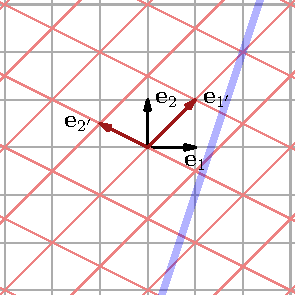
\includegraphics{figuras/plano_coordenadas_rect_trayectoria.pdf}
    \end{figbox}

    Vamos a calcular la distancia entre los puntos de la trayectoria dados por \(t=0\) y \(t=1\). En las coordenadas grises, \(\dot{x}^1 = 1\) y \(\dot{x}^2 = 3\), de modo que el módulo de la velocidad es \(||\mathbf{v}|| = \sqrt{(\dot{x}^1)^2+(\dot{x}^2)^2} = \sqrt{10}\). Así, la longitud del fragmento de la trayectoria es, sencillamente,
    \begin{equation*}
        \ell = \int_0^1\mathrm{d}t\, \sqrt{10} = \sqrt{10}.
    \end{equation*}
    Este resultado no debería sorprender a nadie; un alumno de secundaria podría haber llegado al mismo valor con el teorema de Pitágoras. De hecho, al hacer \(||\mathbf{v}|| = \sqrt{(\dot{x}^1)^2+(\dot{x}^2)^2}\) echamos mano de todo nuestro condicionamiento previo respecto al teorema de Pitágoras. Al fin y al cabo, los vectores \(\mathbf{e}_i\) son ortonormales en el dibujo. 
    
    ¿Cómo quedaría todo esto si quisiéramos utilizar las coordenadas rojas \(x^{i'}\)? Aquí ya hay más miga. Dado que la velocidad es un vector, sus componentes transforman según\footnote{Aunque la regla es general, en el caso de los vectores velocidad se corresponde con la regla de la cadena multidimensional.}
    \begin{equation}
        \dot{x}^{i'} = \jcbn{x}{i'}{x}{i} \dot{x}^{i}.
    \end{equation}
    En este caso, acabamos con \(\dot{x}^{1'} = \frac{7}{3}\) y \(\dot{x}^{1'} = \frac{4}{3}\). A partir de estas componentes debe ser posible, de algún modo, llegar al mismo valor de la velocidad. Sin embargo, el intento ingenuo de calcular \(\sqrt{\left(\frac{7}{3}\right)^2+\left(\frac{4}{3}\right)^2}\) no tiene muchas esperanzas. Los vectores \(\mathbf{e}_{i'}\) ni son ortogonales, ni tienen módulo 1. Lo que sí devuelve el mismo resultado es la operación\marginexercise{Comprobar que, efectivamente, el resultado es \(\sqrt{10}\).}
    \begin{equation*}
        ||\mathbf{v}|| = \sqrt{2\left(\dot{x}^{1'}\right)^2 - \frac{1}{2}\dot{x}^{1'}\dot{x}^{2'} - \frac{1}{2}\dot{x}^{2'}\dot{x}^{1'} + \frac{5}{4}\left(\dot{x}^{1'}\right)^2}.
    \end{equation*}
    Los prefactores \(2, -1/2,\) y \(5/4\) no salen de la nada, como podría parecer. Son los \(g_{i'j'}\) que aparecían en la expresión general (\cref{eq.1-longitud_camino}) y tienen un significado claro. Cuando \(i'=j'\), tenemos el módulo al cuadrado de los \(\mathbf{e}_{i'}\). En cambio, cuando \(i'\neq j'\), lo que aparece es el producto escalar\rnote{Producto escalar}{Es una aplicación que toma dos vectores y devuelve un número. Es bilineal y definida positiva. Además, es la estructura adecuada para construir distancias en el sentido geométrico usual (la noción de distancia en matemáticas es más general que en física).} de \(\mathbf{e}_{1'}\) con \(\mathbf{e}_{2'}\).
    
    Imitando la raíz cuadrada tan grande para las coordenadas grises originales, podemos esribir\marginexercise[-1cm]{Es tremendamente importante ser capaz de obtener las componentes \(g_{i'j'}\) a partir de \(g_{ij}\), suponiendo que \(g_{ij}\) son las componentes de un tensor y, por tanto, conocemos su regla de transformación.}
    \begin{equation*}
        ||\mathbf{v}|| = \sqrt{1\left(\dot{x}^{1}\right)^2 - 0\dot{x}^{1}\dot{x}^{2} - 0\dot{x}^{2}\dot{x}^{1} + 1\left(\dot{x}^{1}\right)^2}.
    \end{equation*}
    Las componentes \(g_{ij}\) asociadas son 1 cuando \(i=j\) y \(0\) cuando \(i\neq j\).\footnote{No confundir con la \(\delta\) de Kronecker. La \(\delta\) de Kronecker es otro tipo de tensor y vale lo mismo en todos los sistemas de coordenadas. La métrica no cumple esa propiedad, y lleva información diferente.} Informalmente, se suele denotar como \(g_{ij} = \text{diag}(1, 1)\). En general, dado un cierto espacio base, si existe alguna elección de coordenadas tal que la métrica tiene esa forma, entonces se dice que el espacio es euclídeo, y a dicha métrica se la llama métrica o distancia euclídea; la de toda la vida.
\end{example}

\begin{example}
    {Métrica euclídea sobre \(\mathbb{R}^2\) en coordenadas polares}
    \label{ex.1-metrica_polares_R2}

    De nuevo hablamos de \(\mathbb{R}^2\). En coordenadas cartesianas \(x^i\), la métrica es \(g_{ij}=\mathrm{diag}(1, 1)\). Es instructivo calcular la métrica en coordenadas polares, \(x^{i'}\). Como \(g_{ij}\) tiene dos subíndices, la ley de transformación que generaliza a las \cref{eq.1-transformacion_componentes,eq.1-transformacion_vectores} es
    \begin{bequation}
        \label{eq.1-transformacion_metrica}
        g_{i'j'} = \jcbn{x}{i}{x}{i'}\jcbn{x}{j}{x}{j'} g_{ij}
    \end{bequation}
    Insistimos en que aún no hemos explicado bien el origen de estas reglas de transformación. Cuando lleguemos a las \cref{sec.2tensores,sec.3variedades} se verá la derivación más claramente. Como las coordenadas cartesianas y las polares se relacionan mediante \(x^1 = x^{1'}\cos\left(x^{2'}\right)\) y \(x^1 = x^{1'}\sin\left(x^{2'}\right)\), las derivadas parciales son:
    \begin{align*}
        \jcbn{x}{1}{x}{1'} &= \cos\left(x^{2'}\right), & &&  \jcbn{x}{2}{x}{1'} &= \sin\left(x^{2'}\right),\\
        \jcbn{x}{1}{x}{2'} &= -x^{1'}\sin\left(x^{2'}\right) & \text{y} &&
        \jcbn{x}{2}{x}{2'} &= x^{2'}\cos\left(x^{2'}\right),
    \end{align*}
    igual que en el \cref{ex.1-plano_coordenadas_polar}. Así, las componentes de la métrica en coordenadas polares son
    \begin{align*}
        g_{1'1'} &= \cos^2\left(x^{2'}\right)g_{11} + \sin^2\left(x^{2'}\right)g_{22} = 1,\\
        g_{1'2'} &= g_{2'1'} = -x^{1'}\sin\left(x^{2'}\right)\cos\left(x^{2'}\right)\left(-g_{11} + g_{22}\right) = 0,\\
        g_{2'2'} &= \left(x^{1'}\right)^2\cos^2\left(x^{2'}\right)g_{11} + \left(x^{1'}\right)^2\sin^2\left(x^{2'}\right)g_{22} = \left(x^{1'}\right)^2.
    \end{align*}
    En otras palabras \(g_{i'j'} = \mathrm{diag}\left(1, \left(x^{1'}\right)^2\right)\). Analicemos estas componentes a la luz de los comentarios del final de los \cref{ex.1-plano_coordenadas_rect_trayectoria,ex.1-plano_coordenadas_polar}. El vector polar radial \(\mathbf{e}_{1'}\) tiene módulo 1, mientras que el angular \(\mathbf{e}_{2'}\) mide \(x^{1'}\);\footnote{Habíamos dado algo de intuición al respecto en la \cref{obs.1-bases_no_ortonormales}. La idea es que la velocidad angular \(\dot{x}^{2'}\) no sabe a qué distancia del origen estamos. No puede decirnos cuántos \(\mathrm{m}/\mathrm{s}\) estamos recorriendo, sino solo cuántas vueltas por \(\mathrm{s}\). Necesitamos multiplicarlo por algo que contenga el radio \(x^{1'}\) como factor de conversión a \(\mathrm{m}/\mathrm{s}\). Ese algo es justamente \(\mathbf{e}_{2'}\).} cuadra perfectamente con las componentes que acabamos de hallar. Además, la base asociada a las coordenadas polares es ortogonal, por lo que los términos no diagonales deben anularse tal y como sucede.

    Vamos a intentar darle un poco más de intuición geométrica a las componentes \(g_{i'j'}\) que acabamos de obtener. Si me muevo en la dirección radial, entonces cada unidad que avanzo en \(x^{1'}\) se corresponde con una unidad de distancia(\(\mathrm{m}\), \(\mathrm{cm}\), \(\mathrm{km}\)...) recorrida. Sin embargo, si me desplazo a lo largo de una una circunferencia, cada \(2\pi\) unidades que recorro en \(x^{2'}\) conllevan un distancia real de \(2\pi \times x^{1'}\).\marginexercise{Con esta intuición sobre el significado de las componentes del tensor métrico, escribir el tensor métrico que le corresponde a \(\mathbb{R}^3\) dotado de la métrica euclídea, descrito conn coordenadas esféricas y cilíndricas. Alternativamente, emplear la \cref{eq.1-transformacion_metrica} para llegar al mismo resultado.}
\end{example}

Volviendo a la física, cerramos esta sección explorando la relación que existe entre la longitud de camino, las trayectorias y la mecánica lagrangiana. Vamos a establecer una relación entre la trayectoria que minimiza la longitud de camino entre dos puntos del espacio base y la que sigue una partícula de masa \(m\) que vive en dicho espacio. 

Supongamos que tenemos dos puntos en nuestro espacio base con coordenadas \(x^i(t_1)\) y \(x^i(t_2)\). Además, medimos distancias con el tensor métrico dado por \(g_{ij}\). Queremos deducir la forma de la trayectoria más corta\footnote{O la más larga (habitualmente no), o, en rigor, la que extremiza la longitud.} entre ambos puntos. Así formulado, lo que tenemos entre manos es un problema de cálculo variacional. La solución, como aprendemos en cursos de mecánica analítica, viene dada por las ecuaciones de Euler-Lagrange. El funcional que debemos minimizar es la longitud de camino \(\ell\) de la \cref{eq.1-longitud_camino}. De ahí vemos que nuestro ``lagrangiano'' tendrá que ser 
\begin{equation}
    L_\ell = \sqrt{g_{ij}\dot{x}^i(t) \dot{x}^j(t)},
\end{equation}
y la trayectoria cumplirá
\begin{equation}
    \frac{\mathrm{d}}{\mathrm{d}t} \frac{\partial L_\ell}{\partial \dot{x}^i} = \frac{\partial L_\ell}{\partial x^i}.
\end{equation}
Ciertamente, la raíz cuadrada nos presenta una perspectiva poco alentadora a la hora de tomar derivadas; sería fabuloso deshacerse de ella. A continuación, justificamos cómo podemos eliminar la raíz y llegar a la misma trayectoria con un lagrangiano mucho más familiar.

Aunque no la hemos calculado explícitamente, pensemos de forma genérica en la trayectoria que minimiza \(\ell\), conocida como geodésica. \rnote{Geodésica}{Trayectoria que minimiza la longitud de camino entre dos puntos del espacio. Generaliza el concepto de línea recta en espacios curvos.} En cualquier caso, estará dada por las funciones \(x^i(t)\), que describen el recorrido a medida que avanza el parámetro \(t\). Ahora bien, sin ningún problema podríamos imaginar el mismo camino, recorrido con una cadencia distinta. Podría empezar más rápido, luego frenar un poco. Podría empezar lento y acelerar de manera uniforme. Podría ir dando pequeños acelerones y frenazos. Podríamos recorrer exactamente el mismo camino de maneras muy diversas. Cada una de estas posibilidades es una parametrización particular de la misma trayectoria. Lo importante para nosotros es entender que, independientemente de la parametrización, la longitud de camino \(\ell\) no puede cambiar. Solo depende del recorrido en sí y de la regla de medir que usemos (la métrica). \marginexercise{Con la regla de la cadena, demostrar que la longitud de camino es invariante bajo cambios de parámetro: \(t(\lambda)\).} 

Convencidos de que la parametrización no importa, podemos escoger sin problema una en la que el módulo de la velocidad sea constante.\rnote[-1cm]{Parámetro afín}{Un parámetro afín se relaciona con la longitud de arco \(s\) como \(t = as+b\). Dan lugar a \(||\mathbf{v}|| = \text{const.}\) En concreto, la longitud de arco \(s\) conlleva que  \(||\mathbf{v}|| = 1\).} De hecho, podemos elegir que la velocidad, en módulo, sea igual a 1 en las unidades adecuadas. Si el módulo de la velocidad es 1, entonces da la feliz casualidad de que 
\begin{equation*}
    \sqrt{g_{ij}\dot{x}^i(t)\dot{x}^j(t)} = g_{ij}\dot{x}^i(t)\dot{x}^j(t).
\end{equation*}
Es decir, dará exactamente lo mismo trabajar con la raíz que sin ella. Si, además, multiplicamos la segunda parte por \(m/2\), llegamos a que el lagrangiano es exactamente la energía cinética de una partícula:
\begin{equation}
    \label{eq.1-lagrangiano-libre}
    L = \frac{m}{2}g_{ij}\dot{x}^i\dot{x}^j.
\end{equation}
Basta, pues, con obtener las ecuaciones de Euler-Lagrange para este lagrangiano ``físico'', que se corresponde con una partícula que se mueve libremente (en ausencia de potenciales o fuerzas), pero confinada a cierto espacio base con métrica \(g_{ij}\). Maravilloso.\footnote{En \href{https://physics.stackexchange.com/questions/149082/geodesic-equation-from-variation-is-the-squared-lagrangian-equivalent?noredirect=1&lq=1}{esta pregunta} de Stack Exchange hay dos respuestas que discuten esto mismo, pero con mayor rigor y nivel de detalle.} Impulsados por una oleadada de optimismo, vamos a ver algunos ejemplos. 

\begin{example}
    {Trayectorias geodésicas en una esfera}
    \label{ex.1-geodesica-esfera}
    Vamos a empezar con un espacio base que tenemos ya bastante estudiado, \(S^2\). Una partícula se mueve libremente (sin fuerzas), sobre la superficie de una esfera. ¿Qué trayectoria seguirá? Debemos aplicar las ecuaciones de Euler-Lagrange, pero primero necesitamos fijar unas coordenadas y las componentes de la métrica asociadas. Fijemos las coordenadas angulares esféricas, \(x^1 = \theta\) y \(x^2 = \phi\). Las componentes de la métrica son \(g_{ij} = \mathrm{diag}\left(1, \sin^2\left(x^1\right)\right)\),\footnote{Ambos términos diagonales van, en general, multiplicados por el radio de la esfera al cuadrado. Este caso es para una esfera de radio 1.} de acuerdo con la intuición que desarrollamos en el \cref{ex.1-metrica_polares_R2}. El radio de los meridianos (\(x^2=\mathrm{const.}\)) es 1, mientras que el radio de los paralelos (\(x^1 = \mathrm{const}.\)) es \(\sin(x^1)\). Además, son direcciones ortogonales, por lo que los términos no diagonales se anulan. \marginexercise{Obtener las componentes de la métrica en las coordenadas de ``proyección'' que veíamos en el \cref{ex.1-hemisferio_norte_S2} es de estudiante aplicado... y ya calcular las ecuaciones de Euler-Lagrange ni te cuento.}

    Según lo anterior, el lagrangiano es
    \begin{equation*}
        L = \frac{m}{2}\left[\left(\dot{x}^1\right)^2 + \sin^2\left(x^1\right)\left(\dot{x}^2\right)^2\right] \quad \text{o, también,}\quad
        L = \frac{m}{2}\left[\dot{\theta}^2 + \sin^2(\theta)\dot{\phi}^2\right].
    \end{equation*}
    De aquí, las ecuaciones de movimiento son:
    \begin{align*}
        &\left\{\begin{aligned}
            \frac{\mathrm{d}}{\mathrm{d}t}\frac{\partial L}{\partial \dot{\theta}} &= m\ddot{\theta}\\
            \frac{\partial L}{\partial \theta} &= m\cos(\theta)\sin(\theta) \dot{\phi}^2
        \end{aligned}\right. &&\implies &\ddot{\theta} &= \cos(\theta)\sin(\theta)\dot{\phi}^2, \\
        &\left\{\begin{aligned}
            \frac{\mathrm{d}}{\mathrm{d}t}\frac{\partial L}{\partial \dot{\phi}} &= m\sin^2(\theta)\left[\ddot{\phi} + 2\frac{\dot{\theta}\dot{\phi}}{\tan(\theta)}\right]\\
            \frac{\partial L}{\partial \phi} &= 0
        \end{aligned}\right. &&\implies &\ddot{\phi} &= -2\frac{\dot{\theta}\dot{\phi}}{\tan(\theta)}. 
    \end{align*}
    Las ecuaciones, así tal cual, intimidan un poco. Analicémoslas un poco para ganar intuición. Lo primero es que la de \(\phi\) está relacionada con la conservación de la componente \(z\) del momento angular. En este sistema se conservan todas las componentes, por supuesto. Sin embargo, nuestra elección de coordenadas solo destaca la dirección \(z\). Lo segundo que podemos hacer es estudiar un caso particular. Como condiciones iniciales, \(\theta(0)=\pi/2\), \(\phi(0) = \phi_0\), y \(\dot{\theta}(0)=0\), \(\dot{\phi}(0) = \omega\). Partiendo de ahí, la trayectoria es \(\theta(t) = \pi/2\) y \(\phi(t) = \phi(0) + \omega t\), es decir, vueltas en el ecuador con velocidad angular constante. 
    
    La trayectoria que hemos obtenido es la más sencilla de expresar por nuestra elección de coordenadas, pero nos permite deducir algo más general sobre las geodésicas de la esfera. Son siempre arcos de círculos máximos.\marginexercise{Es intuitivo y no muy complicado, pero vale la pena parar un momento a formular por qué esperamos que siempre sean arcos de círculos máximos.} Un círculo máximo es una circunferencia como el ecuador, que de radio tiene el radio de la propia esfera. Además del ecuador, los meridianos también son ejemplos de círculos máximos. En la \cref{fig.1-geodesicas_esfera} se muestran tres ejemplos adicionales.

    \begin{figbox}
        {Ejemplos de trayectorias geodésicas en la esfera. Se han obtenido directamente como solución del sistema de ecuaciones diferenciales que constituyen las ecuaciones de movimiento. Aunque sus coordenadas \(\theta(t)\) y \(\phi(t)\) no siguen expresiones sencillas, las trayectorias sí son bastante simples.
        \label{fig.1-geodesicas_esfera}}
        \setlength{\unitlength}{1pt}%
\makeatletter%
\let\ASYencoding\f@encoding%
\let\ASYfamily\f@family%
\let\ASYseries\f@series%
\let\ASYshape\f@shape%
\makeatother%
\leavevmode\vbox to 147.541880pt{}%
\kern 148.545630pt%
\special{pdf:0.000000 g}%
\special{pdf:0.000000 G}%
\fontsize{12.000000}{14.400000}\selectfont%
\usefont{\ASYencoding}{\ASYfamily}{\ASYseries}{\ASYshape}%
\ASYalign(-74.272815,73.770940)(-0.500000,-0.500000){\hbox to 0pt{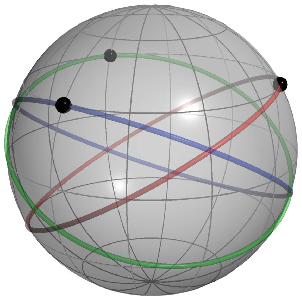
\includegraphics[hiresbb]{./figuras/geodesicas_esfera+0_0.pdf}\hss}%
\includemedia[noplaybutton,3Dlights=Headlamp,3Dmenu,3Dtoolbar=false,label=geodesicas_esfera,3Daac=17.667138151,3Dc2w=0.624695048 -0.780868809 0 -0.232810099 -0.186248079 0.954521404 -0.745355992 -0.596284794 -0.298142397 347.792521305 277.723428875 139.090253081,3Droo=466.300145337,3Dpsob=H,3Dbg=1 1 1,add3Djscript=asylabels.js]{\phantom{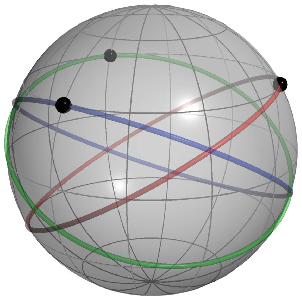
\includegraphics[hiresbb]{./figuras/geodesicas_esfera+0_0.pdf}}}{./figuras/geodesicas_esfera+0.prc}}%

    \end{figbox}

    
\end{example}

\begin{example}
    {Trayectorias geodésicas en un toro \(T^2\) (dónut).}
    Vamos a ver ahora un ejemplo un poco más dulce y picante. Dulce, porque trabajamos ahora sobre la superficie de un dónut, y picante porque ya no es la esfera aburrida que tenemos tan vista. Lo primero es pensar en unas coordenadas adecuadas para un toro. Claramente hay dos circunferencias involucradas; de hecho, el toro es el producto cartesiano de dos circunferencias, \(T^2 = S^1\times S^1\). Esencialmente, tanto si me muevo hacia la derecha como si lo hago hacia arriba, acabo dando vueltas en círculo. Unas buenas coordenadas son, por tanto, los ángulos que determinan la posición dentro de cada circunferencia, \(x^1 = \theta\) y \(x^2 = \phi\).
    
    Podemos visualizar el toro como superficie embebida en el espacio euclídeo,\footnote{Para quien tenga curiosidad, es interesante buscar el ``toro de Clifford'', un \textit{embedding} en \(\mathbb{R}^4\) que, en cierto sentido, es hasta más natural.} \(\mathbb{R}^3\), como en la \cref{fig.1-geodesicas_toro}. Con ese fin, la parametrización habitual es
    \begin{align}
        \left\{\begin{aligned}
            x &= (R + r\sin(\theta))\cos(\phi)\\
            y &= (R + r\sin(\theta))\sin(\phi)\\
            z &= r\cos(\theta)
        \end{aligned}\right.
    \end{align}
    donde \(R\) y \(r\) son los radios que determinan el tamaño del anillo y su grosor, respectivamente. El ángulo \(\phi\) es el azimutal, igual que en esféricas. El ángulo \(\theta\) es ``polar'', pero dentro del dónut.
    
    \begin{figbox}
        {Representación del toro en \(\mathbb{R}^3\). Las trayectorias son geodésicas obtenidas como resultado de integrar las ecuaciones de movimiento.
        \label{fig.1-geodesicas_toro}}
        \setlength{\unitlength}{1pt}%
\makeatletter%
\let\ASYencoding\f@encoding%
\let\ASYfamily\f@family%
\let\ASYseries\f@series%
\let\ASYshape\f@shape%
\makeatother%
\leavevmode\vbox to 66.238330pt{}%
\kern 148.545630pt%
\special{pdf:0.000000 g}%
\special{pdf:0.000000 G}%
\fontsize{12.000000}{14.400000}\selectfont%
\usefont{\ASYencoding}{\ASYfamily}{\ASYseries}{\ASYshape}%
\ASYalign(-74.272815,33.119165)(-0.500000,-0.500000){\hbox to 0pt{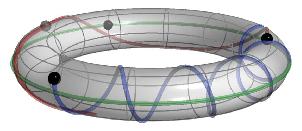
\includegraphics[hiresbb]{./figuras/geodesicas_toro+0_0.pdf}\hss}%
\includemedia[noplaybutton,3Dlights=Headlamp,3Dmenu,3Dtoolbar=false,label=geodesicas_toro,3Daac=9.810391188,3Dc2w=0.624695048 -0.780868809 0 -0.232810099 -0.186248079 0.954521404 -0.745355992 -0.596284794 -0.298142397 288.546518605 230.836040788 110.657052783,3Droo=385.275202595,3Dpsob=H,3Dbg=1 1 1,add3Djscript=asylabels.js]{\phantom{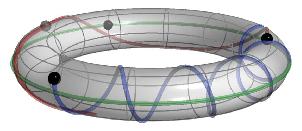
\includegraphics[hiresbb]{./figuras/geodesicas_toro+0_0.pdf}}}{./figuras/geodesicas_toro+0.prc}}%

    \end{figbox}

    Para determinar el lagrangiano, podemos proceder de dos formas, una más geométrica y otra menos. La manera geométrica consiste en partir de la intuición que hemos desarrollado ya sobre lo que significa la métrica. En el caso del toro con las coordenadas elegidas, los elementos no diagonales de \(g\) se anulan, porque los vectores coordenados son ortogonales. En cuanto a los elementos diagonales, debemos tener \(g_{11} = r^2\) y \(g_{22} = \left(R + r\sin(\theta)\right)^2\). Así, llegamos a 
    \begin{equation}
        \label{eq.1-toro_lagrangiano}
        L = \frac{m}{2}\left[r^2 \dot{\theta}^2 + \left(R + r\sin(\theta)\right)^2\dot{\phi}^2\right].
    \end{equation}
    La otra manera\marginexercise{Otro de esos ejercicios recomendables para calentar la muñeca.} consiste en insistir en ver la partícula moviéndose en 3 dimensiones, con velocidad \(||\mathbf{v}||^2 = \dot{x}^2 + \dot{y}^2 + \dot{z}^2\), y utilizar la regla de la cadena para expresar todas esas velocidades en términos de \(\dot{\theta}\) y \(\dot{\phi}\).

    Las ecuaciones de Euler-Lagrange aplicadas a la \cref{eq.1-toro_lagrangiano} son\marginexercise[1cm]{No hay que creerse nada. Obtener las ecuaciones de movimiento de forma explícita.}
    \begin{align*}
        \frac{\mathrm{d}}{\mathrm{d}t}\frac{\partial L}{\partial \dot{\theta}} = \frac{\partial L}{\partial \theta} 
        \quad&\implies\quad
        \ddot{\theta} = \frac{1}{r}\left(R + r\sin(\theta)\right)\cos(\theta)\dot{\phi}^2, 
        \\
        \frac{\mathrm{d}}{\mathrm{d}t}\frac{\partial L}{\partial \dot{\phi}} = \frac{\partial L}{\partial \phi}
        \quad&\implies\quad  \frac{\mathrm{d}}{\mathrm{d}t}\left[\left(R+r\sin(\theta)\right)^2\dot{\phi}\right] = 0.
    \end{align*}
    Si las resolvemos numéricamente, llegamos a las curvas representadas sobre la superficie en la \cref{fig.1-geodesicas_toro}. A pesar de su aspecto, debemos recordar que una partícula que siga dichas trayectorias realmente no siente ninguna aceleración. Más allá del golpe inicial para ponerla en movimiento, no hay nada ``extrínseco'' que la haga moverse, solo obedece a la condición inicial y la curvatura del espacio. 
    
    Alternativamente, podemos ver las trayectorias en el espacio de coordenadas, como en la \cref{fig.1-geodesicas_toro_params}.\marginexercise{Repetir los pasos para un espacio base cilíndrico.} Aquí se ven las mismas tres trayectorias, pero en \([0, 2\pi)\times[0, 2\pi)\in\mathbb{R}^2\). De alguna manera, la moraleja práctica de la geometría diferencial es ser capaces de calcular cosas cuando el espacio base no podemos visualizarlo fácilmente. El espacio de coordenadas es más sencillo de visualizar, porque siempre es un subconjunto de \(\mathbb{R}^n\), como en la \cref{fig.1-geodesicas_toro_params}. Lo que pasa es que, por sí solo, no nos habla de la geometría real del espacio base. Tenemos que complementarla con el tensor métrico, que es quien ``explica'' por qué las trayectorias se curvan de esas formas tan extrañas.
    
    \begin{figbox}
        {Espacio de coordenadas \([0, 2\pi)\times[0, 2\pi)\in\mathbb{R}^2\). Aunque las geodésicas son líneas ``rectas'', aquí se curvan por la curvatura intrínseca del espacio que representa. Las trayectorias, al llegar a un borde, reaparecen por el borde contrario, como en el juego clásico de Pac-Man. \label{fig.1-geodesicas_toro_params}
        }
        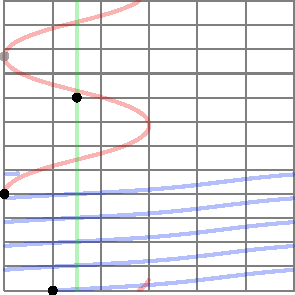
\includegraphics[width=\textwidth]{figuras/geodesicas_toro_params.pdf}
    \end{figbox}
\end{example}

\begin{observation}
    {\textit{Landscape} de trayectorias geodésicas}
    \label{obs.1-geodesica_extremiza}
    Es importante remarcar que las trayectorias no minimizan necesariamente la acción o la longitud de camino, sino que la extremizan. Consideremos la trayectoria roja en las \cref{fig.1-geodesicas_toro,fig.1-geodesicas_toro_params}, entre el punto inicial (negro) y el punto gris. A medida que la partícula se mueve hacia el exterior del toro aumenta el radio de curvatura. Por tanto, es evidente que la trayectoria roja no supone el camino más corto entre ambos extremos; llegaríamos antes por la región interior, con menor radio de curvatura. Tampoco es el camino más largo. Podemos imaginar una trayectoria como la azul que dé muchas vueltas antes de llegar del punto negro al gris.

    Lo que nos dice el principio de acción estacionaria (o de longitud de camino estacionaria, en este caso) es que, una vez fijados el inicio y el final, las trayectorias físicas son aquellas que extremizan la acción. Ahora bien, igual que una función de variable real puede tener varios máximos, mínimos y puntos de inflexión, es posible que haya varias trayectorias que extremicen la acción. Al fin y al cabo, se trata de comparar una trayectoria con otras infinitesimalmente próximas, no con todas las trayectorias posibles; es una comprobación local en el espacio de trayectorias.
    
    De entre todas las trayectorias que extremizan la acción, lo que selecciona la que seguimos son las condiciones iniciales (la velocidad). No todas las velocidades iniciales nos llevarán del punto negro al punto gris, claro, pero todas aquellas que sí nos dejen en el punto gris, lo harán a través de una de estas trayectorias extremas. 
\end{observation}

Antes de pasar a lo siguiente, vamos a calcular la expresión general para las trayectorias a partir del lagrangiano de la \cref{eq.1-lagrangiano-libre}. Se trata de introducirlo en las ecuaciones de Euler-Lagrange que conocemos de mecánica. Eligiendo \(m = 2\) para quitarnos los prefactores molestos,
\begin{equation*}
    \left\{
        \begin{aligned}
            \frac{\mathrm{d}}{\mathrm{d}t}\frac{\partial L}{\partial \dot{x}^{k}} =&\, 
            \frac{\mathrm{d}}{\mathrm{d}t} \left[g_{ij} \frac{\partial \dot{x}^i}{\partial \dot{x}^k} \dot{x}^j +  g_{ij} \dot{x}^i\frac{\partial \dot{x}^j}{\partial \dot{x}^k} \right] = 2\frac{\mathrm{d}}{\mathrm{d}t} \left[g_{jk} \dot{x}^j\right]
            = 2 \partial_i g_{jk} \dot{x}^i \dot{x}^j + 2 g_{jk} \ddot{x}^j\\
            \frac{\partial L}{\partial x^k} =&\, \partial_{k}g_{ij}\dot{x}^i\dot{x}^j
        \end{aligned}
    \right..
\end{equation*}
Uniendo ambos trozos obtenemos
\begin{equation}
    g_{jk} \ddot{x}^j = \frac{1}{2}\left(\partial_{k}g_{ij} - 2 \partial_i g_{jk}\right)\dot{x}^i\dot{x}^j.
\end{equation}
Para terminar de retocar esta expresión, primero observamos que 
\begin{equation*}
    \partial_i g_{jk}\dot{x}^i\dot{x}^j = \partial_j g_{ik}\dot{x}^j\dot{x}^i = \partial_j g_{ik}\dot{x}^i\dot{x}^j, 
\end{equation*}
de modo que
\begin{equation*}
    g_{jk} \ddot{x}^j = \frac{1}{2}\left(\partial_{k}g_{ij} - \partial_i g_{jk} - \partial_j g_{ik}\right)\dot{x}^i\dot{x}^j.
\end{equation*}
Además, multiplicando por la matriz inversa de \(g_{jk}\), que denotaremos por \(g^{lk}\):
\begin{equation}
    \label{eq.1-newton_christoffel}
    \ddot{x}^l = \frac{1}{2}g^{lk}\left(\partial_{k}g_{ij} - \partial_i g_{jk} - \partial_j g_{ik}\right)\dot{x}^i\dot{x}^j.
\end{equation}

Esta expresión representa la ecuación de Newton en un espacio base cualquiera y en coordenadas arbitrarias. El término de la izquierda se corresponde con las ``aceleraciones'', y el de la derecha se corresponde con fuerzas ficticias derivadas de la curvatura. Esta curvatura puede venir del propio espacio base, como en los ejemplos anteriores, o de la elección de coordenadas. Por ejemplo, si utilizamos coordenadas polares para describir \(\mathbb{R}^2\), la métrica tiene coeficientes
\begin{equation}
    g_{rr} = 1,\quad g_{r\theta} = g_{\theta r} = 0\quad\text{y}\quad g_{\theta\theta} = r^2.
\end{equation}
A partir de las componentes de la métrica en este sistema de coordenadas, las ecuaciones de Newton se convierten en \marginexercise{Obtén las ecuaciones siguientes a partir de la \cref{eq.1-newton_christoffel}.}
\begin{equation}
    \left\{\begin{aligned}
        \ddot{r} &= r\dot{\theta}^2\\
        \ddot{\theta} &= -\frac{2}{r}\dot{\theta}\dot{r}
    \end{aligned}\right.
\end{equation}
En la ecuación de \(r\) reconocemos la aceleración centrífuga, mientras que la segunda se puede reorganizar como \(\frac{\mathrm{d}}{\mathrm{d}t}(r^2\dot{\theta}) = 0\), es decir, la conservación del momento angular. 

\subsection{Relatividad especial}
\label{subsec.1relatividad}

En la \cref{subsec.1newton} hemos introducido conceptos de geometría diferencial, nuevo, con la mecánica de newton, conocido, como hilo conductor. Aquí hacemos algo similar. Empezamos hablando de mecánica newtoniana para reformular ciertos términos e ideas de los que normalmente pasamos de largo. Después vemos qué pasa en relatividad especial, donde dichas ideas cobran mucha mayor relevancia.

\subsubsection{Preludio: Galileo}
\label{subsubsec.1galileo}

Solemos pensar en \(\mathbb{R}^3\) como espacio base donde viven nuestras partículas y el tiempo es un parámetro que usamos para describir trayectorias. No obstante, hay algo poco satisfactorio con ver el tiempo como nada más que un parámetro. El tiempo es algo que podemos medir con procesos físicos, mientras que los parámetros son bastante arbitrarios. Por tanto, vamos a meter el tiempo como una dimensión adicional en el espacio base. Así, necesitamos 4 coordenadas, por ejemplo: \(x^0=t\), \(x^1=x\), \(x^2=y\), \(x^3=z\). Para especificar puntos en este espacio base de cuatro dimensiones necesitamos dar los valores de estas cuatro coordenadas. Sin sorpresas hasta aquí.

De todos modos, \(t\) es una coordenada un poco especial. En mecánica newtoniana el tiempo es universal. Para todos los observadores transcurre con la misma cadencia. Si entre dos eventos transcurren 3 tics de un reloj concreto, también transcurrirán 3 tics en cualquier otro reloj, independientemente de cómo se muevan entre sí los relojes. Esto no es así con las coordenadas espaciales. Si yo veo a una señora comer un bocadillo subida a un tren en marcha, entre que lo empieza y lo termina mediré una diferencia de posición \(\Delta x\). Sin embargo, desde el punto de vista de la señora no ha habido ningún desplazamiento entre los mismos sucesos, el que se movía era yo. Lo interesante de que el tiempo sea absoluto es que define una noción de simultaneidad. Si a mí me parece que dos eventos suceden a la vez, también se lo parecerá a la señora del tren. Todo esto resulta muy natural en mecánica newtoniana.

Es común en este tipo de discusiones cambiar el término de ``sistema de coordenadas'' por ``sistema de referencia'', que tiene, quizá, una connotación más física.\footnote{Realmente son conceptos un poco distintos. Un sistema de referencia se refiere a un objeto respecto a cual medimos posiciones. Las coordenadas indican con qué variables expresamos las posiciones.} En concreto, hay una familia de sistemas de referencia especiales. Son aquellos en los que las leyes de Newton tienen validez, y se conocen como sistemas inerciales. En cualquier otro sistema no inercial hay que suplementar las ecuaciones de Newton con términos de ``fuerzas ficticias''.\footnote{Ayuda imaginar lo siguiente. Si estás en un coche que toma una curva, sientes que ``te sales hacia fuera''. La fuerza centrífuga parece bastante real, pero imagina que una cámara fija al techo del coche graba todo lo que sucede y luego ves la grabación. Sin la referencia del exterior (supongamos que las ventanas no son transparentes y no se ve lo que hay fuera), en la grabación se ve a los pasajeros echándose hacia un lado. Para describir su trayectoria \emph{dentro del coche}, necesito incluir una fuerza que los mueva. Esta fuerza no es resultado de ningún proceso físico, es ficticia.} Vamos a ver un par de ejemplos.

\begin{example}
    {Coordenadas no inerciales I}
    \label{ex.1-galileo_noinercial_I}
    Supongamos que tenemos un sistema inercial dado por \((t, x)\), nos olvidamos de \(y\) y \(z\), y una partícula que se desplaza en ausencia de fuerzas siguiendo la trayectoria \(x(t) = vt\). El vector velocidad es \(\mathbf{v} = v\mathbf{e}_x\), y es constante de acuerdo con las leyes de Newton. ¿Qué pasa si cambiamos a las coordenadas \(t' = t, x' = x-\frac{a}{2} t^2\)? ¿Se sigue cumpliendo la ley de Newton en su forma inercial? Es evidente que la trayectoria en el nuevo sistema es \(x' = vt'- \frac{a}{2}(t')^2\) y que la velocidad es \(\mathbf{v}' = \left(v - at'\right)\mathbf{e}_{x'}\).\marginexercise{Estamos usando sin decirlo que \(\mathbf{e}_{x'} = \mathbf{e}_{x}\). Es intuitivo, pero con lo que hemos visto en la \cref{subsec.1transformaciones} podemos incluso demostrarlo explícitamente.} Claramente, el nuevo vector velocidad no es constante, a pesar de que no hay fuerzas externas. Para forzar que la ley de Newton se cumpla debemos añadir una fuerza ficticia igual a \(\mathbf{F}_\mathrm{fict.} = -m a \mathbf{e}_{x'}\).
\end{example}

Este ejemplo ha sido muy sencillo. Está bien para empezar, pero veamos otro más interesante.
\begin{example}
    {Coordenadas no inerciales II}
    \label{ex.1-galileo_noinercial_II}
    Ahora tenemos un sistema inercial dado por \((t, x, y)\), y una partícula que se desplaza en ausencia de fuerzas siguiendo una trayectoria \(x(t) = x(0) + vt\). De nuevo, el vector velocidad es \(\mathbf{v} = v\mathbf{e}_x\), constante. Ahora cambiamos a las coordenadas dadas por la transformación \(t' = t, x' = \cos(\omega t)x + \sin(\omega t)y, y' = -\sin(\omega t)x + \cos(\omega t)y\); hablamos de unas coordenadas que rotan uniformemente en sentido antihorario. Este ejemplo tiene un poco más de miga. Recordemos a donde queremos ir: si las nuevas coordenadas fueran un sistema inercial, tendríamos que el vector velocidad es constante. No sus componentes necesariamente, sino el vector entero. 

    Comencemos invirtiendo el cambio de coordenadas. Debería ser sencillo convencerse de que la transformación inversa es 
    \begin{align*}
        \left\{
        \begin{aligned}
            t &= t'\\
            x &= \cos(\omega t')x' - \sin(\omega t')y'\\
            y &= \sin(\omega t')x' + \cos(\omega t')y'
        \end{aligned}\right..
    \end{align*}
    Con esto, los nuevos vectores coordenados son \(\mathbf{e}_{x'} = \cos(\omega t')\mathbf{e}_x + \sin(\omega t')\mathbf{e}_{y}\) y \(\mathbf{e}_{y'} = -\sin(\omega t')\mathbf{e}_x + \cos(\omega t')\mathbf{e}_x\). Ahora que tenemos toda la información sobre las nuevas coordenadas y sus vectores, transformemos la trayectoria: \(x'(t') = \cos(\omega t') (x(0)+vt')\) e \(y'(t') = -\sin(\omega t') vt'\). Así, la velocidad es \(\mathbf{v}' = v^{x'}\mathbf{e}_{x'}+ v^{y'}\mathbf{e}_{y'}\), y las componentes de la velocidad son
    \begin{align*}
        \left\{
        \begin{aligned}        
            v^{x'} &= \omega \sin(-\omega t')(x(0) + vt') + \cos(-\omega t')v\\
            v^{y'} &= -\omega \cos(-\omega t')(x(0) + vt') + \sin(-\omega t')v
        \end{aligned}
        \right.
    \end{align*}

    
    \begin{figbox}
        {Trayectoria en ausencia de fuerzas externas. Las condiciones iniciales son \(x(0) = -1\), \(y(0) = 0\), \(v^x(0) = 1\), \(v^y(0) = 0\). En la parte superior se toman las coordenadas grises, y se representa con línea punteada el sistema rotante en un instante dado por \(\omega t = 11/5\). En la parte inferior se representa la misma trayectoria vista desde el sistema rotante. 
        \label{fig.1-sistema_rotatorio}}
        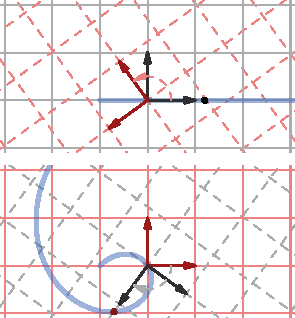
\includegraphics{figuras/sistema_rotatorio.pdf}
    \end{figbox}

    Se puede comprobar que este vector velocidad no cumple las leyes de Newton para una partícula en ausencia de fuerzas externas.\marginexercise[-1cm]{Toma la derivada de las componentes del vector velocidad para llegar a la expresión de la fuerza ficticia. Identifica las fuerzas cetrífuga y de Coriolis.} No hay más que considerar el tipo de trayectorias que representan dichas velocidades. Por ejemplo, miremos la \cref{fig.1-sistema_rotatorio}. Dadas unas condiciones iniciales concretas, se muestra en esta figura la trayectoria de una partícula libre de fuerzas externas. El sistema inercial (líneas grises) presenta una línea recta. En cambio, el otro sistema (líneas rojas) rota respecto al primero, por lo que la trayectoria tiene aspecto de espiral. Un observador subido a dicho sistema de referencia no tiene más remedio que concluir la ``existencia'' de unas fuerzas ficticias.
 
\end{example}

\begin{observation}
    {Sutileza que puede llevar a confusión}
    \label{obs.1-galileo_noinercial}

    Hay un detalle que puede conducir a equívocos sobre qué constituye un sistema no inercial. Supongamos que tenemos un sistema inercial dado por \((t, x, y)\); nos olvidamos de la \(z\), que no importa en esta discusión. Queremos estudiar qué sucede cuando pasamos al sistema dado por las coordenadas polares, \((t, r, \theta)\). ¿Son inerciales estas coordenadas, o tenemos que añadir fuerzas ficticias? Eso es lo que queremos aclarar. La respuesta es que son inerciales, pero es más fácil confundirse de lo que parece. 

    Imaginemos una partícula que sigue la trayectoria dada por \(x = x_0\) e \(y = vt\) en ausencia de fuerzas externas. Claramente, las componentes de la velocidad son constantes \(\dot{x} = 0\) y \(\dot{y} = v\), y se cumplen las leyes de Newton. Genial. ¿Cómo describimos la trayectoria en coordenadas polares? Podemos recurrir a la transformación de coordenadas 
    \begin{align}
        \left\{
        \begin{aligned}
            r &= \sqrt{x^2 + y^2} &&\implies && r(t) = \sqrt{x_0^2 + (vt)^2}\\
            \theta &= \arctan\left(\frac{y}{x}\right) &&\implies && \theta(t) = \arctan\left(\frac{vt}{x_0}\right)
        \end{aligned}\right.,
    \end{align}
    y utilizar la \cref{eq.1-transformacion_componentes}. Alternativamente,\marginexercise{Comprobar que da lo mismo de ambas maneras.} podemos coger \(r(t)\) y \(\theta(t)\) de la expresión anterior para calcular \(v^r=\dot{r}\) y \(v^\theta = \dot{\theta}\) directamente. De cualquier modo,
    \begin{align}
        v^r = \frac{v^2t}{\sqrt{x_0^2 + (vt)^2}}
        \quad\text{y}\quad
        v^{\theta} = \frac{v x_0}{x_0^2 + (vt)^2}.
    \end{align}
    Estas\marginexercise{Integra numéricamente estas ecuaciones y comprueba que, efectivamente, el resultado es una línea recta vertical en \(x=x_0\).} componentes del vector velocidad son claramente no constantes, tal como en el \cref{ex.1-galileo_noinercial_II}. Además no hay fuerzas externas, así que se podría caer en el error de interpretar la dependencia en \(t\) de \(v^{r}\) y \(v^{\theta}\) como una fuerza ficticia, producto de usar un sistema no inercial. Sin embargo, las leyes de Newton no hablan de las componentes de la velocidad, sino del vector velocidad entero. Solo considerando las componentes estaríamos obviando la dependencia temporal de los vectores de la base, inducida por el movimiento de la partícula. En efecto, como vimos en el \cref{ex.1-plano_coordenadas_polar}, los vectores coordenados dependen de la posición en la que se evalúen. A lo largo de la trayectoria,
    \begin{align}
        \left\{\begin{aligned}
            \mathbf{e}_{r}(t) &= \cos\left(\theta(t)\right) \mathbf{e}_{x} + \sin\left(\theta(t)\right) \mathbf{e}_{y}
            \ \text{y}\\
            \mathbf{e}_{\theta}(t) &= -r(t)\sin\left(\theta(t)\right) \mathbf{e}_{x} + r(t)\cos\left(\theta(t)\right) \mathbf{e}_{y}.
        \end{aligned}\right.
    \end{align}
    Si calculamos\marginexercise{Por si había alguna duda, demostrar que \(\frac{\mathrm{d}\mathbf{v}}{\mathrm{d}t} = \mathbf{0}\) queda como ejercicio. Tiene un poquito de truco.} \(\frac{\mathrm{d}\mathbf{v}}{\mathrm{d}t}=\frac{\mathrm{d}}{\mathrm{d}t}\left(v^{r}(t)\mathbf{e}_r(t) + v^{\theta}(t)\mathbf{e}_\theta(t)\right)\), concluiremos que no aparecen fuerzas ficticias.
\end{observation}

El principio de relatividad, dentro de la física newtoniana, habla sobre cómo cambiar de un sistema inercial a otro. La pregunta importante es la siguiente. Dado un sistema inercial, ¿cómo podemos llegar a otros sistemas inerciales? La respuesta técnica son las transformaciones del grupo\rnote{Grupo}{En matemáticas, un grupo es una estructura algebraica formada por un conjunto y una ley de composición. La ley de composición es asociativa, hay un elemento neutro bajo la composición, y todo elemento del conjunto tiene un inverso.} de Galileo. Para que nos entendamos, si desplazamos el origen de coordenadas espaciales o temporal, seguimos en un sistema inercial. Si hacemos una rotación espacial, también. Por último, si pasamos a un sistema que se mueve con respecto a otro inercial con velocidad constante, también estamos en un sistema inercial. En resumen, podemos desplazar, rotar, y mover con velocidad constante. En todos estos sistemas se cumple que, en ausencia de fuerzas externas, el vector velocidad es constante (no necesariamente sus coordenadas). \marginexercise{Comprobar que, dada una trayectoria, cualquiera de estas transformaciones deja el vector velocidad invariante. La regla de la cadena es una amiga.}

Vamos a mirar con calma este último tipo de transformaciones de Galileo. Por simplicidad, supongamos que todo lo interesante sucede en una única dimensión espacial. En ese caso, la transformación que nos lleva de un sistema de referencia (\(t, x\)) a otro (\(t', x'\)) con velocidad relativa \(v\) es \(t' = t\) y \(x' = x - vt\). Los vectores coordenados se relacionan entre sí según la \cref{eq.1-transformacion_vectores}, de manera que \(\mathbf{e}_{x'} = \mathbf{e}_{x}\) y \(\mathbf{e}_{t'} = v\mathbf{e}_{x} + \mathbf{e}_{t}\), como se muestra en la \cref{fig.1-galileo_boost}. Esencialmente es una transformación de ``cizallamiento''.

\begin{figure}[htbp]
    \centering
    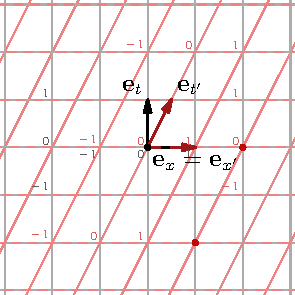
\includegraphics{figuras/galileo_boost.pdf}
    \caption{Líneas coordenadas de los sistemas \(x, t\) y \(x', t'\). Como muestran las etiquetas numéricas, las rectas horizontales se corresponden con \(t=t'=\text{const.}\), mientras que las verticales y oblicuas con \(x=\text{const.}\) y \(x'=\text{const.}\), respectivamente. En un tono más intenso se representan los vectores coordenados.}
    \label{fig.1-galileo_boost}
\end{figure}

Hagamos una cuenta tan sencilla como inútil mirando la figura. Supongamos que \(v = \frac{1}{2}\), como en la \cref{fig.1-galileo_boost}. Entre los dos puntos rojos de la figura hay una separación \(\Delta x = 1\) y \(\Delta t = 2\). En las nuevas coordenadas sabemos que \(\Delta x' = \Delta x - \frac{1}{2} \Delta t=0\) y que \(\Delta t' = \Delta t = 2\). Es como el ejemplo que comentábamos de la señora en el tren. Empieza a comer el bocadillo en el primer punto rojo y acaba en el segundo. Desde su punto de vista, no se ha movido; desde el mío sí. La distancia espacial no es absoluta, sino relativa. En cambio, la distancia temporal es la misma: el tiempo es absoluto. Esta propiedad del tiempo en la física de Newton nos permite definir una distancia espacial en la que todo el mundo está de acuerdo, la distancia entre dos eventos simultáneos. La idea es que, si descomponemos el ``espacio-tiempo'' en lonchas horizontales, todo observador newtoniano piensa en las mismas lonchas temporales.

\subsubsection{Relatividad especial}

Tras la introducción de la \cref{subsubsec.1galileo}, procedemos ahora a hacer una revisión de relatividad especial. Vamos a empezar con una descripción más física para motivar lo que es el verdadero punto de partida en muchas formulaciones modernas. La idea es fijar ciertos conceptos y encontrar relación con lo que hemos visto hasta ahora. Lo primero que debemos hacer es concretar el espacio base de la relatividad especial: el espacio-tiempo de Minkowski. Es un espacio matemático de 4 dimensiones que se corresponden físicamente con el tiempo y las tres dimensiones espaciales, y a los puntos de dicho espacio base se los llama generalmente eventos. 

Hagamos una puntualización. Si necesitamos 4 números reales arbitrarios para describir eventos en el espacio base, ¿por qué no decimos que estamos en \(\mathbb{R}^4\)? ¿Por qué lo llamamos espacio-tiempo de Minkowski, que se denota por \(\mathbb{R}^{3, 1}\)? La respuesta tiene que ver con la cantidad física fundamental que se conserva en este espacio, el intervalo espacio-temporal. Comencemos dando un poco de motivación física sobre la definición del intervalo. Einstein propuso los siguientes postulados: 

\paragraph{Primer postulado (relatividad)} Las leyes de la física toman la misma forma en todos los sistemas de referencia inerciales.

\paragraph{Segundo postulado (invariancia de la velocidad de la luz)} La velocidad de la luz en el vacío, medida en un sistema de referencia inercial, toma siempre el mismo valor denotado por \(c\).

El primer postulado realmente es algo que ya estaba presente en la relatividad galileana de la física de Newton. Lo usábamos para cambiar de un sistema inercial a otro. Lo que cambia es que, ahora, la velocidad de la luz se eleva a la categoría de ley de la naturaleza. Hay otras maneras de plantearlo, y Einstein no era el único que estaba pensando en estas ideas, pero este no es el sitio para tales discusions. Centrémonos en ver a dónde nos lleva esta suposición. Cualquier sistema inercial debe cumplir que la velocidad de la luz es constante. Supongamos que partimos de un sistema inercial \(x^\mu\) con \(\mu = 0, 1, 2, 3\), donde \(x^0 = ct\), \(x^1 = x\), \(x^2 = y\), \(x^3 = z\). Si un objeto parte de un evento con coordenadas \(x_\text{inicial}^\mu\) y se mueve en línea recta a la velocidad de la luz hasta otro punto con coordenadas \(x_\text{final}^\mu\), el espacio que recorre estará relacionado con el tiempo según
\begin{equation*}
    \left(\Delta x\right)^2 + \left(\Delta y\right)^2 + \left(\Delta z\right)^2 = (c\Delta t)^2 
\end{equation*}
También se puede expresar como
\begin{equation}
    \label{eq.1-intervalo_esptemp}
    \left(\Delta s\right)^2 = - \left(\Delta x^0\right)^2 + \left(\Delta x^1\right)^2 + \left(\Delta x^2\right)^2 + \left(\Delta x^3\right)^2 = 0.
\end{equation}
A lo que aparece en la izquierda se lo conoce como intervalo espacio-temporal. Lo que nos dice el segundo postulado es que si describimos los mismos dos eventos en otro sistema también inercial, \(x^{\mu'}\), entonces 
\begin{equation*}
    \left(\Delta s'\right)^{2} = - \left(\Delta x^{0'}\right)^2 + \left(\Delta x^{1'}\right)^2 + \left(\Delta x^{2'}\right)^2 + \left(\Delta x^{3'}\right)^2 = 0.
\end{equation*}
El intervalo espacio-temporal es, por tanto, invariante. Pasemos a la notación de índices sumados, que hace mucho que no la usamos:
\begin{equation}
    \label{eq.1-etamunu}
    \left(\Delta s\right)^2 = \eta_{\mu\nu}\Delta x^\mu \Delta x^\nu = \eta_{\mu'\nu'}\Delta x^{\mu'} \Delta x^{\nu'} = \left(\Delta s'\right)^2,
\end{equation}
donde \(\eta_{\mu\nu}\) son las componentes de un tensor que nos recuerda mucho a la métrica que veíamos en la \cref{subsec.1escalares}. Estrictamente hablando \(\eta_{\mu\nu}\) es una pseudométrica, porque tiene una componente negativa que conduce a propiedades geométricas distintas a las habituales.\rnote[-3.5cm]{Geometría no riemanniana}{Las variedades que hemos tratado en las secciones anteriores tenían una métrica definida positiva, propiedad que define la geometría riemanniana. El espacio-tiempo de la relatividad especial y general es una variedad no riemanniana porque las ``distancias'' que se conservan son los intervalos espacio-temporales.} Aun así, llamaremos a \(\eta_{\mu\nu}\) métrica por comodidad, sin hablar muy alto para que ningún matemático se escandalice. En sistemas inerciales, \(\eta_{\mu\nu} = \text{diag}(-1, 1, 1, 1)\). Como en la \cref{eq.1-etamunu} ambos sistemas son inerciales, entonces \(\eta_{\mu\nu} = \text{diag}(-1, 1, 1, 1) = \eta_{\mu'\nu'}\).

\begin{observation}
    {¿Invariancia o invariancia?}
    \label{obs.1-invariancia}
    Muchos libros introductorios afirman que las transformaciones de Lorentz son aquellas que dejan el intervalo espacio-temporal invariante, pero hay dos sentidos en los que podemos entender ``invariante''. Por un lado, puede ser que la fórmula para calcularlo sea la misma, cambiando \(x^\mu\) por \(x^{\mu'}\).\footnote{O modificaciones triviales por transformaciones ortogonales en las dimensiones espaciales.} Por otro, es posible que la expresión cambie de forma, pero el valor numérico que se obtiene sea el mismo. La invariancia, entendida en el segundo sentido, del intervalo espacio-temporal se cumple siempre porque es un escalar como en la \cref{subsec.1escalares}, independientemente de si las coordenadas son inerciales o no. Ahora bien, en el subconjunto de los sistemas inerciales, el intervalo espacio-temporal tiene la forma de la \cref{eq.1-intervalo_esptemp}, además de coincidir numéricamente.
\end{observation}

Toda la chicha de la relatividad se deriva de la invariancia de \(\left(\Delta s\right)^2\), así que ya hemos terminado con la motivación física... o no. Quien esté atento se dará cuenta de que, por ahora, estamos un poco restringidos a hablar únicamente de eventos entre los que haya un intervalo espacio-temporal nulo. Pero hay muchos pares de puntos que podemos concebir entre los que no hay un \(\left(\Delta s\right)^2 = 0\).\footnote{Este detalle se omite, o no se demuestra, en la gran mayoría de las referencias. Lo importante en relatividad especial es que \(\left(\Delta s\right)^2\) es invariante, y toma la forma de la \cref{eq.1-intervalo_esptemp}, pero habitualmente solo se demuestra que es invariante cuando es igual a cero. Hay más información al respecto \href{https://arxiv.org/abs/0904.3913}{aquí}; es una buena referencia.} Para deshacernos de dicha limitación hay que añadir dos hipótesis razonables.

\paragraph{Homogeneidad del espacio y del tiempo} Todos los puntos del espacio-tiempo son igualmente buenos. Si hago un experimento en un lugar y momento o en otro lugar y otro momento, el resultado debería ser el mismo.  Con esta hipótesis se puede garantizar que las transformaciones entre coordenadas inerciales son lineales,\footnote{Más preciso sería decir ``afines''. Una transformación afín es la composición de una transformación lineal y una traslación. Significa que cambiar el origen de coordenadas tampoco afecta a la física.} es decir, que se pueden expresar como
\begin{equation*}
    x^{\mu'} = \tensor{\Lambda}{^{\mu'}_\mu} x^\mu.
\end{equation*}
El argumento se puede encontrar en el libro de relatividad especial de Wolfgang Rindler, y seguro que en alguno más. Otra manera de justificar la linealidad es que en un sistema de referencia inercial, los objetos se mueven con velocidad constante. Si escojo un sistema de coordenadas no inercial, como el de los \cref{ex.1-galileo_noinercial_I,ex.1-galileo_noinercial_II}, los mismos objetos parecerán moverse bajo la acción de fuerzas ficticias. 

\paragraph{Isotropía del espacio} Todas las direcciones del espacio son equivalentes. Si roto mis ejes, las leyes físicas no cambian. Lo único que cambia es que lo que antes era la dirección \(x\), por ejemplo, ahora se llama de otra manera.

Con estas dos condiciones, se puede demostrar que la invariancia de \(\left(\Delta s\right)^2\) cuando se anula conlleva la invariancia de \(\left(\Delta s\right)^2\) incluso cuando el resultado es distinto de cero. Este resultado es el punto de partida de las formulaciones más directas. A partir de la observación \cref{obs.1-invariancia} podemos deducir qué aspecto tienen las transformaciones de coordenadas que nos llevan de un sistema inercial a otro, análogas a las de Galileo de la \cref{subsubsec.1galileo}. Buscamos una transformación \(\Lambda\) tal que\footnote{Vamos a insistir en algo. Los índices \(\alpha, \beta, \mu, \nu, \mu'\) y \(\nu'\) son mudos. Podemos llamarlos como queramos; se refieren a las coordenadas \(x^0\), \(x^1\), \(x^2\) y \(x^3\) (o las versiones con prima). Hablar de \(x^\alpha\) es lo mismo que hablar de \(x^\mu\). Simplemente cambiamos el nombre al índice según nos convenga para evitar ambigüedades.} 
\begin{equation*}
    \eta_{\mu\nu}\Delta x^\mu \Delta x^\nu = \eta_{\mu'\nu'}\tensor{\Lambda}{^{\mu'}_\alpha} \tensor{\Lambda}{^{\nu'}_\beta}\Delta x^{\alpha} \Delta x^{\beta},
\end{equation*}
donde \(\eta_{\mu\nu} = \text{diag}(-1, 1, 1, 1) = \eta_{\mu'\nu'}\). Como la expresión anterior se debe cumplir para cualquier \(\Delta x^\mu\), tenemos que 
\begin{equation*}
    \eta_{\mu\nu} = \eta_{\mu'\nu'}\tensor{\Lambda}{^{\mu'}_\alpha} \tensor{\Lambda}{^{\nu'}_\beta}.
\end{equation*}

Afortunadamente, el trabajo ya está hecho. La solución es el grupo de Poincaré, que solapa un poco con el grupo de Galileo ya que las traslaciones espacio-temporales\footnote{Las traslaciones no son lineales, sino afines. Si restringimos el grupo de Poincaré a las transformaciones lineales, llegamos al grupo de Lorentz.} y rotaciones espaciales siguen siendo transformaciones entre sistemas inerciales. La diferencia está en cómo trata las transformaciones a sistemas que se mueven con velocidad constante respecto a otro, \textit{boosts} en inglés. La transformación de Lorentz de un \textit{boost} con velocidad \(v\) a lo largo del eje \(X\) tiene las siguientes componentes no nulas
\begin{align}
    \left\{
    \begin{aligned}
        \tensor{\Lambda}{^{ct'}_{ct}} &= \gamma, & \tensor{\Lambda}{^{ct'}_{x}} &= -\gamma \frac{v}{c}, & \tensor{\Lambda}{^{y'}_y} &= 1, \\
        \tensor{\Lambda}{^{x'}_{ct}} &= -\gamma\frac{v}{c}, & \tensor{\Lambda}{^{x'}_{x}} &= \gamma , & \tensor{\Lambda}{^{z'}_z} &= 1, 
    \end{aligned}
    \right.
\end{align}
donde 
\begin{equation}
    \label{eq.1-gamma}
    \gamma = \frac{1}{\sqrt{1-v^2/c^2}} = \frac{1}{\sqrt{1-\beta^2}} \geq 1
\end{equation}
es el factor de Lorentz. Es común referirse a \(v/c\) como \(\beta\). Las coordenadas transversales a la dirección de movimiento no se alteran, mientras que las coordenadas \(x\) y \(ct\) se mezclan de acuerdo a
\begin{align}
    \left\{
    \begin{aligned}
        ct' &= \gamma \left(ct - \beta x\right)\\
        x'  &= \gamma \left(- \beta ct + x\right)
    \end{aligned}
    \right..
\end{align}

Conceptualmente, es importante remarcar que no tenemos por qué usar transformaciones de Lorentz para obtener nuevos sistemas de coordenadas. Pero si queremos que las nuevas coordenadas sean inerciales (que no haya términos de ``fuerzas ficticias'' en las ecuaciones), entonces no queda otra que usar este tipo de transformaciones. En ese sentido, son muy convenientes. El problema conceptual que acarrean es que la mezcla de coordenadas espaciales y temporales induce fenómenos que se salen de la intuición cotidiana. Para ilustrarlos, observemos las líneas coordenadas de la \cref{fig.1-lorentz_boost}. Tanto las líneas grises como las rojo claro cubren todo el espacio-tiempo. Igual que en el caso galileano (\cref{fig.1-galileo_boost}), las líneas de \(x'=\text{const.}\) están inclinadas respecto a la vertical. Sin embargo, las transformaciones de Galileo movían la punta del vector \(\mathbf{e}_t\) a lo largo de una línea horizontal de \(t=t'=\text{const.}\), mientras que ahora también se estira.\footnote{Enfatizamos que es un efecto visual, porque en \(\mathbb{R}^{3,1}\) realmente no hay definida una norma para vectores que tengan componente temporal. Lo que define el espacio-tiempo de Minkowski es una pseudométrica, no una distancia al uso. No tiene sentido calcular el módulo del vector \(\mathbf{e}_{ct'}\) con el teorema de Pitágoras, porque en el espacio-tiempo lo único que funciona es el intervalo espacio-temporal.} Además, las líneas de \(ct'=\text{const.}\) dejan de ser horizontales. Es como si hubiéramos cogido los ejes originales y los hubiésemos acercado de forma simétrica a la bisectriz, en línea discontinua, como cerrando unas tijeras.

Este tipo de transformación ya no es un cizallamiento, sino una rotación hiperbólica. Igual que una rotación ortogonal deja las circunferencias invariantes, la variante hiperbólica deja invariantes las hipérbolas.\marginexercise{Toma la ecuación de una hipérbola arbitraria en las coordenadas \(ct, x\). Transforma las coordenadas y comprueba que la ecuación de la hipérbola sigue cumpliéndose. } Esto significa que si tomamos las coordenadas \(ct, x\) dentro de una hipérbola como la de la \cref{fig.1-lorentz_boost} se convierten en coordenadas de la misma parábola, las coordenadas transformadas \(ct, x\) pertenecen a la misma hipérbola. Aunque se ha propuesto como ejercicio el cálculo directo, es bastante sencillo ver que debe ser así; no es más que otra manera de expresar la invariancia de \((\Delta s)^2\) espacio-temporal.

\begin{figure}[htbp]
    \centering
    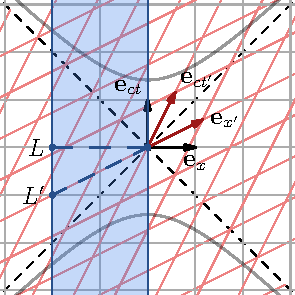
\includegraphics{figuras/lorentz_boost.pdf}
    \caption{Diagrama espacio-temporal. Líneas coordenadas de dos sistemas inerciales relacionados mediante un \textit{boost} con \(\beta=1/2\). Las líneas discontinuas representan trayectorias a la velocidad de la luz que salen del evento central, el cono de luz. La banda azul representa la trayectoria de una barra estacionaria respecto al sistema gris.}
    \label{fig.1-lorentz_boost}
\end{figure}

Las transformaciones de Lorentz tienen consecuencias poco intuitivas. Para ilustrarlas, pensemos en tres situaciones estándar.
\begin{myitemize}
    \item Dilatación temporal. Consideremos los eventos \((ct, x) = (0,0)\) y \((ct, x) = (1, 0)\). Según la \cref{fig.1-lorentz_boost}, en las las nuevas coordenadas tenemos \((ct', x') = (0,0)\) y \((ct', x') = (\gamma ct, -\gamma\beta ct) \simeq (1.155, -0.577)\). Observemos que, igual que con una transformación de Galileo, \(x'<0\) porque el sistema de referencia se mueve hacia la derecha. Sin embargo, tanto el intervalo temporal como el espacial crecen un factor \(\gamma\) respecto a sus contrapartes galileanas. El incremento de \(\Delta ct\) a \(\Delta ct'\) es el conocido efecto de dilatación temporal. 
    \item Relatividad de la simultaneidad. Tomemos los eventos \((ct, x) = (0,0)\) y \((ct, x) = (0, 1)\). En las nuevas coordenadas tenemos \((ct', x') = (0,0)\) y \((ct', x') = (-\gamma\beta x, \gamma x) \simeq (-0.577, 1.155)\). Observemos que los dos eventos tienen la misma coordenada temporal en primer sistema de referencia, son simultáneos. En el segundo sistema, en cambio, las coordenadas temporales son distintas; los mismos dos eventos ya no son simultáneos. En relatividad especial, la noción de simultaneidad ya no es absoluta, como tampoco lo es el tiempo mismo.
    \item Contracción de Lorentz. Los objetos cotidianos tienen dimensiones finitas, no solo hablamos de partículas puntuales. No cuesta nada, por ejemplo, imaginar una barra con cierta longitud. Aun así, en relatividad necesitamos hilar un poco más fino respecto a qué es la longitud de un objeto. Lo primero es reconocer que la longitud de la barra es, realmente, una noción instantánea; ``la barra mide 1 m'' es una afirmación con carácter puramente espacial, donde consideramos los dos extremos simultáneamente. Así expresado, la sutileza ya no es tan sutil: si la noción de simultaneidad es relativa, también debe serlo la longitud de la barra. Al fin y al cabo, los extremos de la barra constituyen dos trayectorias distintas en el espacio-tiempo. Para medir su longitud tenemos que identificar los extremos con dos eventos simultáneos, lo que significa que debemos emplear eventos diferentes según qué sistema de referencia usemos. Volvamos nuestra atención a la banda azul de la \cref{fig.1-lorentz_boost}. Una barra en reposo respecto al sistema gris describe la trayectoria ilustrada en azul, y su longitud es \(L=2\). En cambio, los extremos de la misma barra vistos simultáneamente desde el sistema de referencia rojo claro tienen una separación espacial \(L'=L'/\gamma=\sqrt{3}\simeq 1.732\). Aunque la línea discontinua etiquetada con \(L'\) parezca más larga en la \cref{fig.1-lorentz_boost}, no hay que olvidar que la métrica no es euclídea. La distancia puramente espacial entre el origen y \(L'\) es la que se obtiene contando intersecciones de líneas rojas, de las cuales hay menos de 2. Desde el sistema rojo, la longitud de la barra se reduce.
\end{myitemize}

\paragraph{Intervalo espacio-temporal de una trayectoria arbitraria} Una vez hemos repasado lo más básico de relatividad especial, vamos a conectarlo todo lo visto en las secciones previas. En primer lugar, construimos el intervalo espacio-temporal entre dos eventos conectados por una trayectoria arbitraria \(x^\mu(\lambda)\), donde \(\lambda\) es un parámetro adecuado. Si fraccionamos la trayectoria en pequeños tramos tenemos, para cada uno de ellos, un intervalo espacio-temporal infinitesimal
\begin{equation}
    \label{eq.1-intervalo_esptemp_infinitesimal}
    \mathrm{d}s^2 = \eta_{\mu\nu}\, \mathrm{d}x^\mu \mathrm{d}x^\nu.
\end{equation}
En cada fragmento, \(\mathrm{d}s^2\) puede ser positivo (espacial), negativo (temporal) o cero (nula). Por simplicidad, podemos considerar trayectorias en las que todos los pedazos infinitesimales sean del mismo tipo; afortunadamente, así es para las partículas físicas. Las partículas con masa solo pueden desplazarse mediante trayectorias temporales, mientras que las nulas se reservan a la luz y fenómenos que se propaguen con velocidad \(c\). Las trayectorias espaciales no son realmente físicas. De hecho, una partícula que siga una trayectoria espacial se propagará atrás en el tiempo para algún observador. Para una trayectoria espacial, definimos la longitud espacial como
\begin{subequations}
    \begin{equation}
        \Delta s = \int_{\lambda_1}^{\lambda_2}\mathrm{d}\lambda\, \sqrt{\eta_{\mu\nu} \frac{\mathrm{d}x^\mu}{\mathrm{d}\lambda}\frac{\mathrm{d}x^\nu}{\mathrm{d}\lambda}},
    \end{equation}
    muy similar a la \cref{eq.1-longitud_camino}. En cambio, si la trayectoria es temporal, se define el \textit{tiempo propio} como
    \begin{equation}
        c\Delta \tau = \int_{\lambda_1}^{\lambda_2}\mathrm{d}\lambda\, \sqrt{-\eta_{\mu\nu} \frac{\mathrm{d}x^\mu}{\mathrm{d}\lambda}\frac{\mathrm{d}x^\nu}{\mathrm{d}\lambda}}.
    \end{equation}
\end{subequations}
Aquí, \(\Delta \tau\) es el tiempo medido por un observador comóvil con la trayectoria. 

\paragraph{Vectores y 4-vectores} Un asunto al que hemos dedicado cierta atención en la \cref{subsec.1newton} son los vectores. Lo imporante para que una colección de números conformen las componentes de una magnitud vectorial es que, bajo cambios de base, se transformen de una forma concreta (\cref{eq.1-transformacion_componentes}). Nada ha cambiado llegados a este punto. 

Los vectores más simples en los que podemos pensar son aquellos que se obtienen derivando las coordenadas de una trayectoria respecto de su parámetro \(\frac{\mathrm{d}x^\mu(\lambda)}{\mathrm{d}\lambda}\). La elección de parámetro es libre, dentro de unos márgenes muy generosos. Así, construimos vectores tangentes a cualquier trayectoria. Para partículas masivas existe una elección de parámetro especialmente conveniente: el tiempo propio \(\tau\). La propiedad distintiva de \(\tau\) es que se corresponde con un observable físico en el que cualquier observador está de acuerdo. Además, al tener dimensiones de tiempo, las componentes del vector tangente se identifican con una velocidad física.

Dado un observador inercial en reposo con la trayectoria es evidente que las componentes espaciales se anulan,
\begin{equation*}
    \frac{\mathrm{d}x^{1, 2, 3}}{\mathrm{d}\tau} = 0,
\end{equation*}
porque la trayectoria está en reposo. En cambio, la coordenada temporal aumenta precisamente al ritmo de \(c\). Por tanto, un observador inercial en reposo instantáneo obtiene 
\begin{equation}
    v^\mu = \frac{\mathrm{d}x^\mu}{\mathrm{d}\tau} = (c, 0, 0, 0).
\end{equation}
Este vector \(\mathbf{v} = v^\mu \mathbf{e}_\mu\) se conoce como 4-velocidad.

Para expresar este vector en otro sistema inercial, debemos volver a la \cref{eq.1-transformacion_componentes} y recordar que las nuevas coordenadas se siguen de una transformación de Lorentz:\marginexercise{Desarrollar explícitamente esta expresión para un \textit{boost} en la dirección \(X\).}
\begin{equation}
    v^{\mu'} = \jcbn{x}{\mu'}{x}{\mu} v^{\mu} = \tensor{\Lambda}{^{\mu'}_\mu} v^{\mu}.
\end{equation}
Desempaquetando las sumas implícitas llegamos, para un \textit{boost} de velocidad \(v\) en la dirección \(X\), a
\begin{align*}
    \begin{aligned}
        v^{\mu'} = \frac{\mathrm{d}x^{\mu'}}{\mathrm{d}\tau} = (\gamma c, -\gamma v, 0, 0).
    \end{aligned}
\end{align*}
Ahora bien, estas componentes no se corresponden con la velocidad ``medida'' en el sistema nuevo; al menos no en el sentido habitual. El motivo es claro. La velocidad relativa entre el sistema nuevo y la trayectoria es, realmente, \(\frac{\mathrm{d}x^{1'}}{\mathrm{d}x^{0'}}=-v\), sin la \(\gamma\).\marginexercise{Comprobar que \(\frac{\mathrm{d}x^{1'}}{\mathrm{d}x^{0'}}=-v\) con la regla de la cadena.}

\begin{observation}
    {Sobre el tiempo propio en la 4-velocidad.}
    \label{obs.1-4_velocidad}
    Hay cierta reticencia a parametrizar trayectorias con el tiempo \(x^0\) del observador de referencia. El motivo que se suele dar para evitarlo es que las componentes \(c\frac{\mathrm{d}x^{\mu}}{\mathrm{d}x^{0}}\) no forman un vector como sí lo hacen \(\frac{\mathrm{d}x^{\mu}}{\mathrm{d}\tau}\), porque \(x^0\) no es un invariante relativista mientras que \(\tau\) sí.

    Bien. Hay una pequeña confusión conceptual en lo anterior. Es verdad que \(x^0\) no es invariante y que \(\tau\) sí,\marginexercise{Otro cálculo directo con interés: comprobar que \(c\frac{\mathrm{d}x^{\mu}}{\mathrm{d}x^{0}}\) y \(c\frac{\mathrm{d}x^{\mu'}}{\mathrm{d}x^{0'}}\) no se relacionan con una transformación de Lorentz.} y que si comparásemos \(c\frac{\mathrm{d}x^{\mu}}{\mathrm{d}x^{0}}\) con \(c\frac{\mathrm{d}x^{\mu'}}{\mathrm{d}x^{0'}}\), comprobaríamos que no están relacionadas por \(\tensor{\Lambda}{^{\mu'}_\mu}\). Sin embargo, lo cierto es que \(c\frac{\mathrm{d}x^{\mu}}{\mathrm{d}x^{0}}\) sí forman las componentes de un vector. El problema al pasar de \(c\frac{\mathrm{d}x^{\mu}}{\mathrm{d}x^{0}}\) a \(c\frac{\mathrm{d}x^{\mu'}}{\mathrm{d}x^{0'}}\) es que no estamos usando el mismo parámetro para describir la trayectoria. Si usáramos el mismo parámetro, \(\lambda=x^0\), tendríamos que calcular las componentes 
    \(c\frac{\mathrm{d}x^{\mu}}{\mathrm{d}x^{0}}\) y \(c\frac{\mathrm{d}x^{\mu'}}{\mathrm{d}x^{0}}\), que sí se relacionan mediante \(\tensor{\Lambda}{^{\mu'}_\mu}\). Aun así, tiene cierto sentido físico utilizar un parámetro respecto del cual no hay discusión. Si todos acordamos usar el tiempo propio, en ningún momento habrá riesgo de confusión.
\end{observation}

Queda establecido que la 4-velocidad es un vector. A partir de vectores y el tensor métrico, podemos construir escalares como vimos en la \cref{subsec.1escalares}. En concreto, ahora es pertinente escribir \(\eta_{\mu\nu}v^{\mu}v^\nu\). Si queremos averiguar cuánto vale esta expresión, debemos escoger un sistema de referencia para llevar a cabo el cálculo. Elijamos uno en reposo con la trayectoria, de modo que \(v^\mu=(c, 0, 0, 0)\). Entonces,
\begin{equation}
    \eta_{\mu\nu}v^{\mu}v^\nu = -c^2.
\end{equation}
Como \(\eta_{\mu\nu}v^{\mu}v^\nu\) es un invariante,\footnote{¡Invariante respecto a cambios de coordenadas generales! No solo transformaciones de Lorentz, como se puede encontrar escrito por ahí.} el mismo\marginexercise{Comprueba que se llega al mismo resultado (i) en un sistema inercial arbitrario, y (ii) en un sistema de coordenadas arbitrario.} cálculo repetido en cualquier sistema de referencia llevará al mismo resultado. 

A continuación, es oportuno plantearse cómo cambia la ley de adición de velocidades. Según la relatividad galileana, si un sistema inercial \(S''\) se mueve respecto a otro \(S'\), que a su vez se desplaza respecto a \(S\), entonces \(S''\) se mueve respecto a \(S\) con la suma algebraica de las velocidades involucradas. En física relativista, la invariancia de la velocidad de la luz conlleva un cambio en esta regla. Consideremos dos sistemas inerciales \(S\) y \(S'\) relacionados por un \textit{boost} de velocidad \(v\) en la dirección \(X\), y además otro sistema \(S''\) relacionado con \(S'\) mediante otro \textit{boost} de velocidad \((u^{x'}, u^{y'}, u^{z'})\). La pregunta es con qué velocidad, \((u^{x}, u^{y}, u^{z})\), se desplaza \(S''\) respecto de \(S\). Podemos averiguar la respuesta simplemente componiendo dos \textit{boosts} de Lorentz consecutivos:
\begin{equation}
    x^{\mu''} = \tensor{\Lambda}{^{\mu''}_{\mu'}}\tensor{\Lambda}{^{\mu'}_{\mu}} x^\mu = \tensor{\Lambda}{^{\mu''}_{\mu}} x^\mu,
\end{equation}
pero es un camino largo y lleno de espinas.\marginexercise{Un poquito de sufrimiento nunca está de más. Calcular la composición de \textit{boosts} y extraer la ley de adición de velocidades en el caso colineal.} Es más sencillo plantearlo del siguiente modo.

La 4-velocidad de \(S'\) respecto de \(S\) es \(v^\mu = (\gamma_v c, \gamma_v v, 0, 0)\), y la 4-velocidad de \(S''\) respecto de \(S'\) es \(w^{\mu'} = (\gamma_{u'} c, \gamma_{u'} u^{x'}, \gamma_{u'} u^{y'}, \gamma_{u'} u^{z'})\), donde \(\gamma_v\) o \(\gamma_{u'}\) son los factores de Lorentz asociados a \(v\) y a \(u'\), respectivamente. Para expresar las componentes \(w^{\mu'}\) en el sistema \(S\) debemos calcular
\begin{equation}
    w^{\mu} = \tensor{\Lambda}{^{\mu}_{\mu'}} w^{\mu'} = (\gamma_u c, \gamma_u u^{x}, \gamma_u u^{y}, \gamma_u u^{z}),
\end{equation}
donde \(\tensor{\Lambda}{^\mu_{\mu'}}\) no es más que un \textit{boost} con velocidad \(-v\) en la dirección \(X\). De aquí se deduce que 
\begin{align}
    \left\{
    \begin{aligned}
        w^{ct} &= \gamma_v\gamma_{u'}\left(c + \frac{v u^{x'}}{c}\right)=\gamma_{u} c, & w^{x} &= \gamma_v \gamma_{u'}(v + u^{x'}) = \gamma_u u^x, \\
        w^{y} &= \gamma_{u'} u^{y'}=\gamma_{u} u^{y}, & w^{z} &= \gamma_{u'} u^{z'}=\gamma_{u} u^{z}.
    \end{aligned}
    \right.
\end{align}
Ahora el objetivo es despejar las componentes \((u^{x}, u^{y}, u^{z})\).\marginexercise{No vamos a darlo todo hecho. Comprobar que las expresiones siguientes son correctas.} Con pocos malabares algebraicos se llega a 
\begin{align}
    \begin{aligned}
        u^{x} &= \frac{u^{x'} + v}{1 + \frac{u^{x'} v}{c^2}}, & u^{y,z} &= \frac{u^{y',z'}}{\gamma_v \left(1 + \frac{v u^{x'}}{c^2}\right)}.
    \end{aligned}
\end{align}
He aquí la ley de adición de velocidades relativista, bastante más compleja que su análogo galileano.

Al hilo de la observación anterior, y a la luz de la ley de adición de velocidades, uno puede concluir que las componentes \(u^{i} = c\frac{\mathrm{d}x^i}{\mathrm{d}x^0}\) con \(i = 1, 2, 3\) no se transforman en \(u^{i'}\) como lo harían las componentes de un vector. No obstante, repetimos de nuevo, esto no significa que \(c\frac{\mathrm{d}x^\mu}{\mathrm{d}x^0} = (c, u^x, u^y, u^z)\) no sea un 4-vector. Lo que pasa es que no podemos esperar transformar las coordenadas y, a la vez, cambiar el parámetro sin que haya diferencia respecto de transformar únicamente las coordenadas. Formalmente, tan buen parámetro es \(x^0\) como \(x^{0'}\) o \(\tau\). Mientras usemos siempre el mismo, la transformación de las componentes será de Lorentz. Otra cuestión es qué significado otorgamos a dichas componentes. 

Lo último que nos queda por discutir relacionado con la 4-velocidad es su relación con otro vector célebre, el 4-momento. Si tomamos la 4-velocidad y la multiplicamos por un escalar seguimos teniendo un 4-vector. Es así, de hecho, como se construye el 4-momento:
\begin{equation}
    \label{eq.1-4momento}
    p^\mu = m v^\mu = (\gamma m c, \gamma m v^x, \gamma m v^y, \gamma m v^z).
\end{equation}
Es una relación idéntica a la que hay entre la velocidad y el momento cinético ``usuales'', pero ahora las componentes llevan factores de \(\gamma\) dentro. En concreto, \(p^{ct} = \gamma mc = \frac{E}{c}\) se identifica con el contenido energético de la partícula debido a su masa y su movimiento.\footnote{La identidad \(E = \gamma mc^2\), o su versión en reposo, \(E_0=mc^2\) está tan arraigada en el imaginario colectivo que casi da vergüenza cuestionarse si \(\gamma mc^2\) tiene derecho a interpretarse como energía. Esta es, sin embargo, una pregunta legítima. Se pueden ver justificaciones en el libro de Landau y Lifshitz \textit{La teoría clásica de campos}, o en \textit{El significado de la relatividad}, del propio Einstein.} Por supuesto, el estatus de \(p^\mu\) de componentes de un vector implica propiedades de transformación agradables entre sistemas de referencia inerciales. 

\paragraph{Tensor de Faraday o de campo electromagnético} Por último, veamos rápidamente ejemplos de tensores en la teoría física que dio paso a todo el asunto de la relatividad: la electrodinámica.\footnote{Las pistas sobre la relatividad venían de las leyes del electromagnetismo, que no son invariantes bajo transformaciones de Galileo, pero sí bajo las de Lorentz.} En formulaciones modernas de electrodinámica, los grados de libertad electromagnéticos quedan recogidos en el 4-potencial.\rnote[-1.5cm]{1-forma diferencial}{Así escrito, \(A_\mu\) son las componentes de una 1-forma diferencial, nombre dado a los covectores en el espacio cotangente de una variedad diferencial. Se puede poner en correspondencia biunívoca con un vector de componentes \(A^\mu\) mediante \(A_\mu = \eta_{\mu\nu}A^\nu\).}
\begin{equation}
    A_\mu = \left(-\frac{\phi}{c}, A^x, A^y, A^z\right),
\end{equation}
formado por los potenciales escalar y vector. A partir de \(A_\mu\) se define el tensor de Faraday, con componentes\rnote[1.5cm]{Derivada exterior}{Operador en geometría diferencial que lleva un tensor antisimétrico de rango \((0,k)\) en otro, también asimétrico y de rango \((0,k+1)\). El nombre se lo debe a su comportamiento, que generaliza el de una derivada.}
\begin{equation}
    F_{\mu\nu} = \frac{\partial A_\nu}{\partial x^\mu} - \frac{\partial A_\mu}{\partial x^\nu} = \partial_\mu A_\nu - \partial_\nu A_\mu. 
\end{equation}
En términos de los\marginexercise{Convencerse de que el tensor de Faraday es antisimétrico y obtener sus componentes en términos de los campos eléctrico y magnético.} campos electromagnéticos habituales,\footnote{¡Los índices en \(F_{ii}\) no están sumados!}
\begin{align*}
    \left\{
    \begin{aligned}
        F_{0,\nu} &= \left(0, -\frac{E_x}{c}, -\frac{E_y}{c}, -\frac{E_z}{c}\right),\\
        F_{i,i} &= 0,\\
        F_{i,j} &= \varepsilon_{ijk}B_k.
    \end{aligned}\right.
\end{align*}

Ahora podríamos preguntarnos cómo transformar los campos eléctricos y magnéticos de un sistema inercial a otro. Con argumentos físicos complicados acabaríamos llegando a un resultado; siendo optimistas al correcto. El poder de la formulación geométrica de la física relativista es que \(F_{\mu\nu}\) son las componentes de un tensor y, por tanto, se transforman según\footnote{Ya lo hemos dicho, pero repetimos que la ley de transformación general es válida también para
transformaciones que no sean de Lorentz. Lo que pasa es que con las de Lorentz la forma de las ecuaciones se mantiene, cumplen el principio de covariancia o invariancia, aunque algunos autores especifican ``invariancia de forma''.}
\begin{equation*}
    F_{\mu'\nu'} = \jcbn{x}{\mu}{x}{\mu'}\jcbn{x}{\nu}{x}{\nu'} F_{\mu'\nu'} \underset{\text{Lorentz}}{=} \tensor{\Lambda}{^\mu_{\mu'}}\tensor{\Lambda}{^\nu_{\nu'}} F_{\mu\nu},
\end{equation*}
prescindiendo de razonamientos enrevesados.\marginexercise{Demostrar que, en el sentido espacial, el campo magnético \(\mathbf{B}\) es un pseudovector (o vector axial).} Desarrollando las sumas implícitas para un \textit{boost} de velocidad \(\mathbf{v} = (v^x, v^y, v^z)\) se llega a
\begin{subequations}
    \label{eq.1-EB_lorentz}
    \begin{align}
        \text{(paralelo a \(\mathbf{v}\))}&\left\{
        \begin{aligned}
            \mathbf{E}_\parallel ' &= \mathbf{E}_\parallel  \\
            \mathbf{B}_\parallel ' &= \mathbf{B}_\parallel
        \end{aligned}\right.,\\
        \text{(perpendicular a \(\mathbf{v}\))}&\left\{
        \begin{aligned}
            \mathbf{E}_\perp ' &= \gamma\left(\mathbf{E}_\perp + \mathbf{v}\times\mathbf{B}\right)  \\
            \mathbf{B}_\perp ' &= \gamma\left(\mathbf{B}_\perp - \frac{1}{c^2}\mathbf{v}\times\mathbf{E}\right)
        \end{aligned}\right..
    \end{align}
\end{subequations}
Estas reglas de transformación indican que una combinación de campos electromagnéticos en un sistema inercial se corresponde con una combinación diferente en otro sistema. Su aspecto debería confirmar algo que ya hemos notado: los campos \(\mathbf{E}\) y \(\mathbf{B}\) no son magnitudes vectoriales en el sentido de la geometría diferencial en el espacio-tiempo de Minkowski. Para empezar, solo tienen 3 componentes en lugar de 4, pero es que las reglas de transformación entre sistemas inerciales no coinciden con una sola transformación de Lorentz. 

\begin{example}
    {Campo electromagnético de una carga puntual}
    \label{ex.1-campo_em_carga}

    Hay muchos efectos electromagnéticos que se pueden entender con mayor profundidad aprovechando la \cref{eq.1-EB_lorentz}. Aquí únicamente vamos a representar el campo electromagnético de una carga puntual estacionaria o en movimiento respecto a un sistema inercial. Fijemos una ``loncha'' temporal en \(\mathbb{R}^{3, 1}\) usando el tiempo de un sistema de coordenadas inercial \(x^{\mu}\). En este ``fotograma'', una carga puntual \(q\) en reposo situada en \(\mathbf{r}_q = (x_q, y_q, z_q)\) da lugar únicamente al campo eléctrico de Coulomb
    \begin{equation}
        \mathbf{E}(\mathbf{r}) = \frac{q}{4\pi\varepsilon_0 |\mathbf{r}-\mathbf{r}_q|^3} (\mathbf{r}-\mathbf{r}_q),
    \end{equation}
    y \(\mathbf{B}(\mathbf{r})=\mathbf{0}\). ¿Qué campo veremos para una carga en movimiento en el mismo evento espacio-temporal? A partir de la \cref{eq.1-EB_lorentz} parece trivial, pero hay una sutileza de esas que son obvias a posteriori.\footnote{Las notas de David Tong, disponibles en \href{https://davidtong.org/teaching/}{su página web}, son siempre muy recomendables. Ahora mismo nos interesa el capítulo de electromagnetismo y relatividad de sus notas de electromagnetismo.}

    Sea \(\mathbf{v}=(v, 0, 0)\) la velocidad de la carga relativa al sistema \(x^{\mu}\). Desde el sistema inercial \(x^{\mu'}\), donde la carga está en reposo, tenemos una situación idéntica a la anterior. Los campos eléctrico y magnético se expresan de manera trivial, para un punto arbitrario del espacio-tiempo, en términos de las coordenadas comóviles \(x^{\mu'} = (ct', \mathbf{r}')\):
    \begin{subequations}
        \begin{align}
            \label{eq.1-E_moving}
            \mathbf{E}'(\mathbf{r}') &= \frac{q}{4\pi\varepsilon_0 |\mathbf{r}'-\mathbf{r}'_q|^3} (\mathbf{r}'-\mathbf{r}'_q),\\
            \mathbf{B}'(\mathbf{r}') &= \mathbf{0}.
        \end{align}
    \end{subequations}
    Como los sistemas \(x^{\mu'}\) y \(x^{\mu}\) se relacionan mediante un \textit{boost} de velocidad \(-\mathbf{v}\), recurrimos a la \cref{eq.1-EB_lorentz} para transformar las componentes de los campos. De este modo, \(\mathbf{E}_\parallel(\mathbf{r}') = \mathbf{E}_\parallel'(\mathbf{r}')\) y \(\mathbf{E}_\perp(\mathbf{r}') = \gamma\mathbf{E}_\perp'(\mathbf{r}')\), por ejemplo; hasta aquí todos de acuerdo.
    
    Nos falta, sin embargo, un último paso. Si queremos expresar las componentes de los campos vistas desde el sistema \(x^\mu\), entonces también tendremos que usar estas coordenadas para expresar la posición del evento espacio-temporal. En otras palabras, para un evento dado, no solo hay que transformar las componentes, sino también cambiar las coordenadas que asignamos a dicho evento. En otras palabras, queremos pasar de \(\mathbf{E}(\mathbf{r}')\) a \(\mathbf{E}(\mathbf{r})\). Las coordenadas se relacionan mediante
    \begin{align}
        ct' = \gamma(ct - \beta x), && x' = \gamma(-\beta ct + x), && y' = y, && z' = z,
    \end{align}
    donde \(\beta=v/c\). 
    
    Avancemos paso a paso. El 3-vector \(\mathbf{r}' - \mathbf{r}_q'\) que aparece en la \cref{eq.1-E_moving} se expresa, en términos de las coordenadas \(x^\mu\) como 
    \begin{equation}
        \label{eq.1-positions_rest_coordinates}
        \mathbf{r}' - \mathbf{r}'_q = \left(\gamma(x-x_q), y-y_q, z-z_q\right) = \left(\gamma(x-vt), y-y_q, z-z_q\right)
    \end{equation}
    Es razonablemente obvio que \(x_q = \beta ct = vt\): en \(x^{\mu}\) la carga se mueve hacia la derecha con velocidad \(v\), y suponemos, sin perder generalidad, que en \(t=0\) teníamos \(x_q = 0\). El factor \(\gamma\) en la primera coordenada confabula con los factores \(\gamma\) que aparecen en las componentes transversales \(\mathbf{E}_\perp\) (\cref{eq.1-EB_lorentz}). Como consecuencia aparece un factor \(\gamma\) que multiplica a toda la expresión del campo eléctrico \(\mathbf{E}\), que mantiene la dirección radial con centro la posición de la carga. Trasladando la \cref{eq.1-positions_rest_coordinates} al denominador de \cref{eq.1-E_moving} llegamos a
    \begin{equation*}
        \mathbf{E}(\mathbf{r}) = \frac{\gamma q \left(x-vt, y-y_q, z-z_q\right)}{4\pi\varepsilon_0\Big[\gamma^2(x-vt)^2 + (y-y_q)^2 + (z-z_q)^2\Big]^{3/2}}.
    \end{equation*}
    A pesar de ser un campo radial, existe una diferencia importante respecto al campo de una carga estática: los factores \(\gamma\). Analicemos sus implicaciones. Para el campo en la dirección de movimiento, el módulo de campo eléctrico se reduce un factor \(\gamma^2\). Es razonable, porque estamos evaluando el campo en una posición ``contraída''. En cambio, en las direcciones transversales el campo se incrementa en un factor \(\gamma\). En consecuencia, las líneas de campo eléctrico de una carga en movimiento dejan de presentar simetría esférica, como sucedía con cargas estacionarias, y pasan a una disposición esferoidal achatada en la dirección de movimiento.\footnote{En la jerga habitual se repite el término \textit{pancake}.}

    En cuanto al campo magnético de la carga en movimiento uniforme, tenemos
    \begin{equation}
        \mathbf{B}(\mathbf{r}) = \gamma\frac{1}{c^2}\mathbf{v}\times\mathbf{E}(\mathbf{r}).
    \end{equation}
    Es perpendicular al campo eléctrico y a la velocidad de la partícula, de modo que forma líneas de campo circulares alrededor del eje de movimiento. La \cref{fig.1-EB_lorentz} muestra dos cargas, una estática y otra con velocidad uniforme. La primera emana un campo eléctrico radial e isótropo, mientras que en el otro caso vemos la forma de \textit{pancake}, junto con el vector campo magnético asociado.
    \begin{figbox}[0.5]
        {Dos cargas, una estática y otra en movimiento uniforme, junto con su campo electromagnético. El campo eléctrico de la carga estática es el de Coulomb, radial e isótropo. La otra carga tiene un campo eléctrico contraído en la dirección \(X\), y estirado en las otras direcciones. Las líneas de campo magnético rodean la partícula.
        \label{fig.1-EB_lorentz}}
        \setlength{\unitlength}{1pt}%
\makeatletter%
\let\ASYencoding\f@encoding%
\let\ASYfamily\f@family%
\let\ASYseries\f@series%
\let\ASYshape\f@shape%
\makeatother%
\leavevmode\vbox to 124.455680pt{}%
\kern 177.654320pt%
\special{pdf:0.000000 g}%
\special{pdf:0.000000 G}%
\fontsize{12.000000}{14.400000}\selectfont%
\usefont{\ASYencoding}{\ASYfamily}{\ASYseries}{\ASYshape}%
\ASYalign(-88.827160,62.227840)(-0.500000,-0.500000){\hbox to 0pt{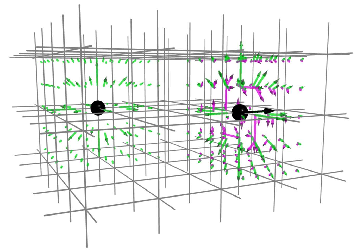
\includegraphics[hiresbb]{./figuras/EB_lorentz+0_0.pdf}\hss}%
\includemedia[noplaybutton,3Dlights=Headlamp,3Dmenu,3Dtoolbar=false,label=EB_lorentz,3Daac=34.037827876,3Dc2w=0.894427191 -0.447213595 0 -0.059467182 -0.118934365 0.991119706 -0.443242207 -0.886484414 -0.132972662 82.338521757 182.421574735 19.01295378,3Droo=200.737994043,3Dpsob=H,3Dbg=1 1 1,add3Djscript=asylabels.js]{\phantom{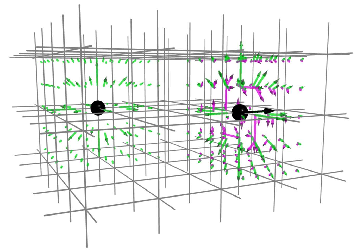
\includegraphics[hiresbb]{./figuras/EB_lorentz+0_0.pdf}}}{./figuras/EB_lorentz+0.prc}}%

    \end{figbox}

\end{example}

Con este ejemplo concluimos nuestro paseo inicial por las ideas y notación de la geometría diferencial. Hemos ido de la mano de la física, que da un poco de sabor a nociones matemáticas que, de otro modo, pueden dejarle a uno un poco frío. Las siguientes secciones van más al grano en lo que se refiere a definiciones y conceptos. Habrá, también, referencias a la física para que no se nos haga tan seco, pero el balance será más inclinado hacia las matemáticas que hasta ahora. 